\documentclass[12pt,a4paper,oneside,]{article}
\def\ifdoblecara{} %% set to true
\let\ifdoblecara\undefined %% set to false
\def\ifprincipal{} %% set to true
\def\ifcitapandoc{} %% set to true
\let\ifcitapandoc\undefined %% set to false
\usepackage{lmodern}
% sin fontmathfamily
\usepackage{amssymb,amsmath}
\usepackage{ifxetex,ifluatex}
%\usepackage{fixltx2e} % provides \textsubscript %PLLC
\ifnum 0\ifxetex 1\fi\ifluatex 1\fi=0 % if pdftex
  \usepackage[T1]{fontenc}
  \usepackage[utf8]{inputenc}
\else % if luatex or xelatex
  \ifxetex
    \usepackage{mathspec}
  \else
    \usepackage{fontspec}
  \fi
  \defaultfontfeatures{Ligatures=TeX,Scale=MatchLowercase}
\fi
% use upquote if available, for straight quotes in verbatim environments
\IfFileExists{upquote.sty}{\usepackage{upquote}}{}
% use microtype if available
\IfFileExists{microtype.sty}{%
\usepackage{microtype}
\UseMicrotypeSet[protrusion]{basicmath} % disable protrusion for tt fonts
}{}
\usepackage[margin = 2.5cm]{geometry}
\usepackage{hyperref}
\hypersetup{unicode=true,
              pdfborder={0 0 0},
              breaklinks=true}
\urlstyle{same}  % don't use monospace font for urls
    \usepackage{natbib}
  \bibliographystyle{apa-good}
  \usepackage[usenames,dvipsnames]{xcolor}  %new PLLC
\usepackage{color}
\usepackage{fancyvrb}
\newcommand{\VerbBar}{|}
\newcommand{\VERB}{\Verb[commandchars=\\\{\}]}
\DefineVerbatimEnvironment{Highlighting}{Verbatim}{commandchars=\\\{\}}
% Add ',fontsize=\small' for more characters per line
\usepackage{framed}
\definecolor{shadecolor}{RGB}{248,248,248}
\newenvironment{Shaded}{\begin{snugshade}}{\end{snugshade}}
\newcommand{\AlertTok}[1]{\textcolor[rgb]{0.94,0.16,0.16}{#1}}
\newcommand{\AnnotationTok}[1]{\textcolor[rgb]{0.56,0.35,0.01}{\textbf{\textit{#1}}}}
\newcommand{\AttributeTok}[1]{\textcolor[rgb]{0.77,0.63,0.00}{#1}}
\newcommand{\BaseNTok}[1]{\textcolor[rgb]{0.00,0.00,0.81}{#1}}
\newcommand{\BuiltInTok}[1]{#1}
\newcommand{\CharTok}[1]{\textcolor[rgb]{0.31,0.60,0.02}{#1}}
\newcommand{\CommentTok}[1]{\textcolor[rgb]{0.56,0.35,0.01}{\textit{#1}}}
\newcommand{\CommentVarTok}[1]{\textcolor[rgb]{0.56,0.35,0.01}{\textbf{\textit{#1}}}}
\newcommand{\ConstantTok}[1]{\textcolor[rgb]{0.00,0.00,0.00}{#1}}
\newcommand{\ControlFlowTok}[1]{\textcolor[rgb]{0.13,0.29,0.53}{\textbf{#1}}}
\newcommand{\DataTypeTok}[1]{\textcolor[rgb]{0.13,0.29,0.53}{#1}}
\newcommand{\DecValTok}[1]{\textcolor[rgb]{0.00,0.00,0.81}{#1}}
\newcommand{\DocumentationTok}[1]{\textcolor[rgb]{0.56,0.35,0.01}{\textbf{\textit{#1}}}}
\newcommand{\ErrorTok}[1]{\textcolor[rgb]{0.64,0.00,0.00}{\textbf{#1}}}
\newcommand{\ExtensionTok}[1]{#1}
\newcommand{\FloatTok}[1]{\textcolor[rgb]{0.00,0.00,0.81}{#1}}
\newcommand{\FunctionTok}[1]{\textcolor[rgb]{0.00,0.00,0.00}{#1}}
\newcommand{\ImportTok}[1]{#1}
\newcommand{\InformationTok}[1]{\textcolor[rgb]{0.56,0.35,0.01}{\textbf{\textit{#1}}}}
\newcommand{\KeywordTok}[1]{\textcolor[rgb]{0.13,0.29,0.53}{\textbf{#1}}}
\newcommand{\NormalTok}[1]{#1}
\newcommand{\OperatorTok}[1]{\textcolor[rgb]{0.81,0.36,0.00}{\textbf{#1}}}
\newcommand{\OtherTok}[1]{\textcolor[rgb]{0.56,0.35,0.01}{#1}}
\newcommand{\PreprocessorTok}[1]{\textcolor[rgb]{0.56,0.35,0.01}{\textit{#1}}}
\newcommand{\RegionMarkerTok}[1]{#1}
\newcommand{\SpecialCharTok}[1]{\textcolor[rgb]{0.00,0.00,0.00}{#1}}
\newcommand{\SpecialStringTok}[1]{\textcolor[rgb]{0.31,0.60,0.02}{#1}}
\newcommand{\StringTok}[1]{\textcolor[rgb]{0.31,0.60,0.02}{#1}}
\newcommand{\VariableTok}[1]{\textcolor[rgb]{0.00,0.00,0.00}{#1}}
\newcommand{\VerbatimStringTok}[1]{\textcolor[rgb]{0.31,0.60,0.02}{#1}}
\newcommand{\WarningTok}[1]{\textcolor[rgb]{0.56,0.35,0.01}{\textbf{\textit{#1}}}}

% PLLC modifica-ini
% PLLC modifica-fin

\IfFileExists{parskip.sty}{%
\usepackage{parskip}
}{% else
\setlength{\parindent}{0pt}
\setlength{\parskip}{6pt plus 2pt minus 1pt}
}
\setlength{\emergencystretch}{3em}  % prevent overfull lines
\providecommand{\tightlist}{%
  \setlength{\itemsep}{0pt}\setlength{\parskip}{0pt}}
\setcounter{secnumdepth}{5}
% Redefines (sub)paragraphs to behave more like sections
\ifx\paragraph\undefined\else
\let\oldparagraph\paragraph
\renewcommand{\paragraph}[1]{\oldparagraph{#1}\mbox{}}
\fi
\ifx\subparagraph\undefined\else
\let\oldsubparagraph\subparagraph
\renewcommand{\subparagraph}[1]{\oldsubparagraph{#1}\mbox{}}
\fi

%%% Use protect on footnotes to avoid problems with footnotes in titles
\let\rmarkdownfootnote\footnote%
\def\footnote{\protect\rmarkdownfootnote}


  \title{}
    \author{}
    \date{}
  

%%%%%%% inicio: latex_preambulo.tex PLLC


%% UTILIZA CODIFICACIÓN UTF-8
%% MODIFICARLO CONVENIENTEMENTE PARA USARLO CON OTRAS CODIFICACIONES


%\usepackage[spanish,es-nodecimaldot,es-noshorthands]{babel}
\usepackage[spanish,es-nodecimaldot,es-noshorthands,es-tabla]{babel}
% Ver: es-tabla (en: https://osl.ugr.es/CTAN/macros/latex/contrib/babel-contrib/spanish/spanish.pdf)
% es-tabla (en: https://tex.stackexchange.com/questions/80443/change-the-word-table-in-table-captions)
 
\usepackage{float}
\usepackage{placeins}
\usepackage{fancyhdr}
% Solucion: ! LaTeX Error: Command \counterwithout already defined.
% https://tex.stackexchange.com/questions/425600/latex-error-command-counterwithout-already-defined
\let\counterwithout\relax
\let\counterwithin\relax
\usepackage{chngcntr}
%\usepackage{microtype}  %antes en template PLLC
\usepackage[utf8]{inputenc}
\usepackage[T1]{fontenc} % Usa codificación 8-bit que tiene 256 glyphs

%\usepackage[dvipsnames]{xcolor}
%\usepackage[usenames,dvipsnames]{xcolor}  %new
\usepackage{pdfpages}
%\usepackage{natbib}




% Para portada: latex_paginatitulo_mod_ST02.tex (inicio)
\usepackage{tikz}
\usepackage{epigraph}
\input{portadas/latex_paginatitulo_mod_ST02_add.sty}
% Para portada: latex_paginatitulo_mod_ST02.tex (fin)

% Para portada: latex_paginatitulo_mod_OV01.tex (inicio)
\usepackage{cpimod}
% Para portada: latex_paginatitulo_mod_OV01.tex (fin)

% Para portada: latex_paginatitulo_mod_OV03.tex (inicio)
\usepackage{KTHEEtitlepage}
% Para portada: latex_paginatitulo_mod_OV03.tex (fin)

\renewcommand{\contentsname}{Índice}
\renewcommand{\listfigurename}{Índice de figuras}
\renewcommand{\listtablename}{Índice de tablas}
\newcommand{\bcols}{}
\newcommand{\ecols}{}
\newcommand{\bcol}[1]{\begin{minipage}{#1\linewidth}}
\newcommand{\ecol}{\end{minipage}}
\newcommand{\balertblock}[1]{\begin{alertblock}{#1}}
\newcommand{\ealertblock}{\end{alertblock}}
\newcommand{\bitemize}{\begin{itemize}}
\newcommand{\eitemize}{\end{itemize}}
\newcommand{\benumerate}{\begin{enumerate}}
\newcommand{\eenumerate}{\end{enumerate}}
\newcommand{\saltopagina}{\newpage}
\newcommand{\bcenter}{\begin{center}}
\newcommand{\ecenter}{\end{center}}
\newcommand{\beproof}{\begin{proof}} %new
\newcommand{\eeproof}{\end{proof}} %new
%De: https://texblog.org/2007/11/07/headerfooter-in-latex-with-fancyhdr/
% \fancyhead
% E: Even page
% O: Odd page
% L: Left field
% C: Center field
% R: Right field
% H: Header
% F: Footer
%\fancyhead[CO,CE]{Resultados}

%OPCION 1
% \fancyhead[LE,RO]{\slshape \rightmark}
% \fancyhead[LO,RE]{\slshape \leftmark}
% \fancyfoot[C]{\thepage}
% \renewcommand{\headrulewidth}{0.4pt}
% \renewcommand{\footrulewidth}{0pt}

%OPCION 2
% \fancyhead[LE,RO]{\slshape \rightmark}
% \fancyfoot[LO,RE]{\slshape \leftmark}
% \fancyfoot[LE,RO]{\thepage}
% \renewcommand{\headrulewidth}{0.4pt}
% \renewcommand{\footrulewidth}{0.4pt}
%%%%%%%%%%
\usepackage{calc,amsfonts}
% Elimina la cabecera de páginas impares vacías al finalizar los capítulos
\usepackage{emptypage}
\makeatletter

%\definecolor{ocre}{RGB}{25,25,243} % Define el color azul (naranja) usado para resaltar algunas salidas
\definecolor{ocre}{RGB}{0,0,0} % Define el color a negro (aparece en los teoremas

%\usepackage{calc} 


%era if(csl-refs) con dolares
% metodobib: true


\usepackage{lipsum}

%\usepackage{tikz} % Requerido para dibujar formas personalizadas

%\usepackage{amsmath,amsthm,amssymb,amsfonts}
\usepackage{amsthm}


% Boxed/framed environments
\newtheoremstyle{ocrenumbox}% % Theorem style name
{0pt}% Space above
{0pt}% Space below
{\normalfont}% % Body font
{}% Indent amount
{\small\bf\sffamily\color{ocre}}% % Theorem head font
{\;}% Punctuation after theorem head
{0.25em}% Space after theorem head
{\small\sffamily\color{ocre}\thmname{#1}\nobreakspace\thmnumber{\@ifnotempty{#1}{}\@upn{#2}}% Theorem text (e.g. Theorem 2.1)
\thmnote{\nobreakspace\the\thm@notefont\sffamily\bfseries\color{black}---\nobreakspace#3.}} % Optional theorem note
\renewcommand{\qedsymbol}{$\blacksquare$}% Optional qed square

\newtheoremstyle{blacknumex}% Theorem style name
{5pt}% Space above
{5pt}% Space below
{\normalfont}% Body font
{} % Indent amount
{\small\bf\sffamily}% Theorem head font
{\;}% Punctuation after theorem head
{0.25em}% Space after theorem head
{\small\sffamily{\tiny\ensuremath{\blacksquare}}\nobreakspace\thmname{#1}\nobreakspace\thmnumber{\@ifnotempty{#1}{}\@upn{#2}}% Theorem text (e.g. Theorem 2.1)
\thmnote{\nobreakspace\the\thm@notefont\sffamily\bfseries---\nobreakspace#3.}}% Optional theorem note

\newtheoremstyle{blacknumbox} % Theorem style name
{0pt}% Space above
{0pt}% Space below
{\normalfont}% Body font
{}% Indent amount
{\small\bf\sffamily}% Theorem head font
{\;}% Punctuation after theorem head
{0.25em}% Space after theorem head
{\small\sffamily\thmname{#1}\nobreakspace\thmnumber{\@ifnotempty{#1}{}\@upn{#2}}% Theorem text (e.g. Theorem 2.1)
\thmnote{\nobreakspace\the\thm@notefont\sffamily\bfseries---\nobreakspace#3.}}% Optional theorem note

% Non-boxed/non-framed environments
\newtheoremstyle{ocrenum}% % Theorem style name
{5pt}% Space above
{5pt}% Space below
{\normalfont}% % Body font
{}% Indent amount
{\small\bf\sffamily\color{ocre}}% % Theorem head font
{\;}% Punctuation after theorem head
{0.25em}% Space after theorem head
{\small\sffamily\color{ocre}\thmname{#1}\nobreakspace\thmnumber{\@ifnotempty{#1}{}\@upn{#2}}% Theorem text (e.g. Theorem 2.1)
\thmnote{\nobreakspace\the\thm@notefont\sffamily\bfseries\color{black}---\nobreakspace#3.}} % Optional theorem note
\renewcommand{\qedsymbol}{$\blacksquare$}% Optional qed square
\makeatother




% Define el estilo texto theorem para cada tipo definido anteriormente
\newcounter{dummy} 
\numberwithin{dummy}{section}
\theoremstyle{ocrenumbox}
\newtheorem{theoremeT}[dummy]{Teorema}  % (Pedro: Theorem)
\newtheorem{problem}{Problema}[section]  % (Pedro: Problem)
\newtheorem{exerciseT}{Ejercicio}[section] % (Pedro: Exercise)
\theoremstyle{blacknumex}
\newtheorem{exampleT}{Ejemplo}[section] % (Pedro: Example)
\theoremstyle{blacknumbox}
\newtheorem{vocabulary}{Vocabulario}[section]  % (Pedro: Vocabulary)
\newtheorem{definitionT}{Definición}[section]  % (Pedro: Definition)
\newtheorem{corollaryT}[dummy]{Corolario}  % (Pedro: Corollary)
\theoremstyle{ocrenum}
\newtheorem{proposition}[dummy]{Proposición} % (Pedro: Proposition)


\usepackage[framemethod=default]{mdframed}



\newcommand{\intoo}[2]{\mathopen{]}#1\,;#2\mathclose{[}}
\newcommand{\ud}{\mathop{\mathrm{{}d}}\mathopen{}}
\newcommand{\intff}[2]{\mathopen{[}#1\,;#2\mathclose{]}}
\newtheorem{notation}{Notation}[section]


\mdfdefinestyle{exampledefault}{%
rightline=true,innerleftmargin=10,innerrightmargin=10,
frametitlerule=true,frametitlerulecolor=green,
frametitlebackgroundcolor=yellow,
frametitlerulewidth=2pt}


% Theorem box
\newmdenv[skipabove=7pt,
skipbelow=7pt,
backgroundcolor=black!5,
linecolor=ocre,
innerleftmargin=5pt,
innerrightmargin=5pt,
innertopmargin=10pt,%5pt
leftmargin=0cm,
rightmargin=0cm,
innerbottommargin=5pt]{tBox}

% Exercise box	  
\newmdenv[skipabove=7pt,
skipbelow=7pt,
rightline=false,
leftline=true,
topline=false,
bottomline=false,
backgroundcolor=ocre!10,
linecolor=ocre,
innerleftmargin=5pt,
innerrightmargin=5pt,
innertopmargin=10pt,%5pt
innerbottommargin=5pt,
leftmargin=0cm,
rightmargin=0cm,
linewidth=4pt]{eBox}	

% Definition box
\newmdenv[skipabove=7pt,
skipbelow=7pt,
rightline=false,
leftline=true,
topline=false,
bottomline=false,
linecolor=ocre,
innerleftmargin=5pt,
innerrightmargin=5pt,
innertopmargin=10pt,%0pt
leftmargin=0cm,
rightmargin=0cm,
linewidth=4pt,
innerbottommargin=0pt]{dBox}	

% Corollary box
\newmdenv[skipabove=7pt,
skipbelow=7pt,
rightline=false,
leftline=true,
topline=false,
bottomline=false,
linecolor=gray,
backgroundcolor=black!5,
innerleftmargin=5pt,
innerrightmargin=5pt,
innertopmargin=10pt,%5pt
leftmargin=0cm,
rightmargin=0cm,
linewidth=4pt,
innerbottommargin=5pt]{cBox}

% Crea un entorno para cada tipo de theorem y le asigna un estilo 
% con ayuda de las cajas coloreadas anteriores
\newenvironment{theorem}{\begin{tBox}\begin{theoremeT}}{\end{theoremeT}\end{tBox}}
\newenvironment{exercise}{\begin{eBox}\begin{exerciseT}}{\hfill{\color{ocre}\tiny\ensuremath{\blacksquare}}\end{exerciseT}\end{eBox}}				  
\newenvironment{definition}{\begin{dBox}\begin{definitionT}}{\end{definitionT}\end{dBox}}	
\newenvironment{example}{\begin{exampleT}}{\hfill{\tiny\ensuremath{\blacksquare}}\end{exampleT}}		
\newenvironment{corollary}{\begin{cBox}\begin{corollaryT}}{\end{corollaryT}\end{cBox}}	

%	ENVIRONMENT remark
\newenvironment{remark}{\par\vspace{10pt}\small 
% Espacio blanco vertical sobre la nota y tamaño de fuente menor
\begin{list}{}{
\leftmargin=35pt % Indentación sobre la izquierda
\rightmargin=25pt}\item\ignorespaces % Indentación sobre la derecha
\makebox[-2.5pt]{\begin{tikzpicture}[overlay]
\node[draw=ocre!60,line width=1pt,circle,fill=ocre!25,font=\sffamily\bfseries,inner sep=2pt,outer sep=0pt] at (-15pt,0pt){\textcolor{ocre}{N}}; \end{tikzpicture}} % R naranja en un círculo (Pedro)
\advance\baselineskip -1pt}{\end{list}\vskip5pt} 
% Espaciado de línea más estrecho y espacio en blanco después del comentario


\newenvironment{solutionExe}{\par\vspace{10pt}\small 
\begin{list}{}{
\leftmargin=35pt 
\rightmargin=25pt}\item\ignorespaces 
\makebox[-2.5pt]{\begin{tikzpicture}[overlay]
\node[draw=ocre!60,line width=1pt,circle,fill=ocre!25,font=\sffamily\bfseries,inner sep=2pt,outer sep=0pt] at (-15pt,0pt){\textcolor{ocre}{S}}; \end{tikzpicture}} 
\advance\baselineskip -1pt}{\end{list}\vskip5pt} 

\newenvironment{solutionExa}{\par\vspace{10pt}\small 
\begin{list}{}{
\leftmargin=35pt 
\rightmargin=25pt}\item\ignorespaces 
\makebox[-2.5pt]{\begin{tikzpicture}[overlay]
\node[draw=ocre!60,line width=1pt,circle,fill=ocre!55,font=\sffamily\bfseries,inner sep=2pt,outer sep=0pt] at (-15pt,0pt){\textcolor{ocre}{S}}; \end{tikzpicture}} 
\advance\baselineskip -1pt}{\end{list}\vskip5pt} 

\usepackage{tcolorbox}

\usetikzlibrary{trees}

\theoremstyle{ocrenum}
\newtheorem{solutionT}[dummy]{Solución}  % (Pedro: Corollary)
\newenvironment{solution}{\begin{cBox}\begin{solutionT}}{\end{solutionT}\end{cBox}}	


\newcommand{\tcolorboxsolucion}[2]{%
\begin{tcolorbox}[colback=green!5!white,colframe=green!75!black,title=#1] 
 #2
 %\tcblower  % pone una línea discontinua
\end{tcolorbox}
}% final definición comando

\newtcbox{\mybox}[1][green]{on line,
arc=0pt,outer arc=0pt,colback=#1!10!white,colframe=#1!50!black, boxsep=0pt,left=1pt,right=1pt,top=2pt,bottom=2pt, boxrule=0pt,bottomrule=1pt,toprule=1pt}



\mdfdefinestyle{exampledefault}{%
rightline=true,innerleftmargin=10,innerrightmargin=10,
frametitlerule=true,frametitlerulecolor=green,
frametitlebackgroundcolor=yellow,
frametitlerulewidth=2pt}





\newcommand{\betheorem}{\begin{theorem}}
\newcommand{\eetheorem}{\end{theorem}}
\newcommand{\bedefinition}{\begin{definition}}
\newcommand{\eedefinition}{\end{definition}}

\newcommand{\beremark}{\begin{remark}}
\newcommand{\eeremark}{\end{remark}}
\newcommand{\beexercise}{\begin{exercise}}
\newcommand{\eeexercise}{\end{exercise}}
\newcommand{\beexample}{\begin{example}}
\newcommand{\eeexample}{\end{example}}
\newcommand{\becorollary}{\begin{corollary}}
\newcommand{\eecorollary}{\end{corollary}}


\newcommand{\besolutionExe}{\begin{solutionExe}}
\newcommand{\eesolutionExe}{\end{solutionExe}}
\newcommand{\besolutionExa}{\begin{solutionExa}}
\newcommand{\eesolutionExa}{\end{solutionExa}}


%%%%%%%%


% Caja Salida Markdown
\newmdenv[skipabove=7pt,
skipbelow=7pt,
rightline=false,
leftline=true,
topline=false,
bottomline=false,
backgroundcolor=GreenYellow!10,
linecolor=GreenYellow!80,
innerleftmargin=5pt,
innerrightmargin=5pt,
innertopmargin=10pt,%5pt
innerbottommargin=5pt,
leftmargin=0cm,
rightmargin=0cm,
linewidth=4pt]{mBox}	

%% RMarkdown
\newenvironment{markdownsal}{\begin{mBox}}{\end{mBox}}	

\newcommand{\bmarkdownsal}{\begin{markdownsal}}
\newcommand{\emarkdownsal}{\end{markdownsal}}


\usepackage{array}
\usepackage{multirow}
\usepackage{wrapfig}
\usepackage{colortbl}
\usepackage{pdflscape}
\usepackage{tabu}
\usepackage{threeparttable}
\usepackage{subfig} %new
%\usepackage{booktabs,dcolumn,rotating,thumbpdf,longtable}
\usepackage{dcolumn,rotating}  %new
\usepackage[graphicx]{realboxes} %new de: https://stackoverflow.com/questions/51633434/prevent-pagebreak-in-kableextra-landscape-table

%define el interlineado vertical
%\renewcommand{\baselinestretch}{1.5}

%define etiqueta para las Tablas o Cuadros
%\renewcommand\spanishtablename{Tabla}

%%\bibliographystyle{plain} %new no necesario


%%%%%%%%%%%% PARA USO CON biblatex
% \DefineBibliographyStrings{english}{%
%   backrefpage = {ver pag.\adddot},%
%   backrefpages = {ver pags.\adddot}%
% }

% \DefineBibliographyStrings{spanish}{%
%   backrefpage = {ver pag.\adddot},%
%   backrefpages = {ver pags.\adddot}%
% }
% 
% \DeclareFieldFormat{pagerefformat}{\mkbibparens{{\color{red}\mkbibemph{#1}}}}
% \renewbibmacro*{pageref}{%
%   \iflistundef{pageref}
%     {}
%     {\printtext[pagerefformat]{%
%        \ifnumgreater{\value{pageref}}{1}
%          {\bibstring{backrefpages}\ppspace}
%          {\bibstring{backrefpage}\ppspace}%
%        \printlist[pageref][-\value{listtotal}]{pageref}}}}
% 
%%% de kableExtra
\usepackage{booktabs}
\usepackage{longtable}
%\usepackage{array}
%\usepackage{multirow}
%\usepackage{wrapfig}
%\usepackage{float}
%\usepackage{colortbl}
%\usepackage{pdflscape}
%\usepackage{tabu}
%\usepackage{threeparttable}
\usepackage{threeparttablex}
\usepackage[normalem]{ulem}
\usepackage{makecell}
%\usepackage{xcolor}

%%%%%%% fin: latex_preambulo.tex PLLC


\begin{document}



% nada
\begin{titlepage}

\newcommand{\HRule}{\rule{\linewidth}{0.5mm}} % Defines a new command for the horizontal lines, change thickness here

\center % Center everything on the page


\begin{minipage}{14cm}
%----------------------------------------------------------------------------------------
%  LOGO SECTION
%----------------------------------------------------------------------------------------
\center

\includegraphics[width=8cm,height=8cm]{logo}\\[0.5cm] % Include a department/university logo - this will require the graphicx package

%----------------------------------------------------------------------------------------

%----------------------------------------------------------------------------------------
%	HEADING SECTIONS
%----------------------------------------------------------------------------------------
\textsc{\LARGE Grado ...}\\[2.5cm] 


%----------------------------------------------------------------------------------------
%	TITLE SECTION
%----------------------------------------------------------------------------------------

\rule[1.7mm]{2cm}{0.5mm}
\hfill
\textsc{\Large TRABAJO FIN DE ESTUDIOS} 
\hfill
\rule[1.7mm]{2cm}{0.5mm} 
\\[0.75cm]

%\bfseries
{\Huge
\textbf{\textit{
Introducción a \\[0.2cm]
la Estadística Aplicada \\[0.5cm]
con ayuda de R
}}}\\[0.75cm] 

\HRule \\[4cm]


{\Large

Marta García Moreno} \\[0.5cm]

{\large
Sevilla, Octubre de 2017
}

\end{minipage}

\vfill % Fill the rest of the page with whitespace

\cleardoublepage
%\newpage{\ }
\thispagestyle{empty}
\end{titlepage}

\raggedbottom




\setlength{\parindent}{1em}

\pagestyle{fancy}
\ifdefined\ifdoblecara
\fancyhead[LE,RO]{}
\fancyhead[LO,RE]{}
\else
\fancyhead[RO]{}
\fancyhead[LO]{}
\fi
\renewcommand{\headrulewidth}{0pt}
\renewcommand{\footrulewidth}{0pt}
\pagenumbering{roman}

\setcounter{tocdepth}{4}
\subpdfbookmark{Índice General}{indice}
\tableofcontents

\cleardoublepage

\section*{Prólogo}
\addcontentsline{toc}{section}{Prólogo}

Escrito colocado al comienzo de una obra en el que se hacen comentarios
sobre la obra o su autor, o se introduce en su lectura; a menudo está
realizado por una persona distinta del autor.

También se podrían incluir aquí los agradecimientos.

\cleardoublepage

\section*{Resumen}
\addcontentsline{toc}{section}{Resumen}

Resumen\ldots{}

\clearpage
\section*{Abstract}
\addcontentsline{toc}{section}{Abstract}

Abstract\ldots{}

\cleardoublepage   
\listoffigures
\addcontentsline{toc}{section}{Índice de Figuras}

\cleardoublepage

\listoftables

\addcontentsline{toc}{section}{Índice de Tablas}

\cleardoublepage

\pagenumbering{arabic}

\ifdefined\ifdoblecara
\fancyhead[LE,RO]{\scriptsize\rightmark}
\fancyfoot[LO,RE]{\scriptsize\slshape \leftmark}
\fancyfoot[C]{}
\fancyfoot[LE,RO]{\footnotesize\thepage}
\else
\fancyhead[RO]{\scriptsize\rightmark}
\fancyfoot[LO]{\scriptsize\slshape \leftmark}
\fancyfoot[C]{}
\fancyfoot[RO]{\footnotesize\thepage}
\fi

\renewcommand{\headrulewidth}{0.4pt}
\renewcommand{\footrulewidth}{0.4pt}

\ifdefined\ifprincipal
\else
\setlength{\parindent}{1em}
\pagestyle{fancy}
\setcounter{tocdepth}{4}
\tableofcontents

\nocite{Luque2017,Luque2019,RStudio,R-base2,
R-knitr,R-rmarkdown,R-dplyr,R-ggplot2,Techopedia}

\fi

\ifdefined\ifdoblecara
\fancyhead{}{}
\fancyhead[LE,RO]{\scriptsize\rightmark}
\fancyfoot[LO,RE]{\scriptsize\slshape \leftmark}
\fancyfoot[C]{}
\fancyfoot[LE,RO]{\footnotesize\thepage}
\else
\fancyhead{}{}
\fancyhead[RO]{\scriptsize\rightmark}
\fancyfoot[LO]{\scriptsize\slshape \leftmark}
\fancyfoot[C]{}
\fancyfoot[RO]{\footnotesize\thepage}
\fi

\renewcommand{\headrulewidth}{0.4pt}
\renewcommand{\footrulewidth}{0.4pt}

\hypertarget{tuxedtulo-del-capuxedtulo}{%
\section{Título del Capítulo}\label{tuxedtulo-del-capuxedtulo}}

\hypertarget{primera-secciuxf3n}{%
\subsection{Primera sección}\label{primera-secciuxf3n}}

\FloatBarrier

\ifdefined\ifprincipal
\else
\setlength{\parindent}{1em}
\pagestyle{fancy}
\setcounter{tocdepth}{4}
\tableofcontents

\nocite{Luque2017,Luque2019,RStudio,R-base2,
R-knitr,R-rmarkdown,R-dplyr,R-ggplot2,Techopedia}

\fi

\ifdefined\ifdoblecara
\fancyhead{}{}
\fancyhead[LE,RO]{\scriptsize\rightmark}
\fancyfoot[LO,RE]{\scriptsize\slshape \leftmark}
\fancyfoot[C]{}
\fancyfoot[LE,RO]{\footnotesize\thepage}
\else
\fancyhead{}{}
\fancyhead[RO]{\scriptsize\rightmark}
\fancyfoot[LO]{\scriptsize\slshape \leftmark}
\fancyfoot[C]{}
\fancyfoot[RO]{\footnotesize\thepage}
\fi

\renewcommand{\headrulewidth}{0.4pt}
\renewcommand{\footrulewidth}{0.4pt}

\hypertarget{tuxedtulo-del-capuxedtulo-1}{%
\section{Título del Capítulo}\label{tuxedtulo-del-capuxedtulo-1}}

\hypertarget{primera-secciuxf3n-1}{%
\subsection{Primera sección}\label{primera-secciuxf3n-1}}

\FloatBarrier

\ifdefined\ifprincipal
\else
\setlength{\parindent}{1em}
\pagestyle{fancy}
\setcounter{tocdepth}{4}
\tableofcontents

\nocite{Luque2017,Luque2019,RStudio,R-base2,
R-knitr,R-rmarkdown,R-dplyr,R-ggplot2,Techopedia}

\fi

\ifdefined\ifdoblecara
\fancyhead{}{}
\fancyhead[LE,RO]{\scriptsize\rightmark}
\fancyfoot[LO,RE]{\scriptsize\slshape \leftmark}
\fancyfoot[C]{}
\fancyfoot[LE,RO]{\footnotesize\thepage}
\else
\fancyhead{}{}
\fancyhead[RO]{\scriptsize\rightmark}
\fancyfoot[LO]{\scriptsize\slshape \leftmark}
\fancyfoot[C]{}
\fancyfoot[RO]{\footnotesize\thepage}
\fi

\renewcommand{\headrulewidth}{0.4pt}
\renewcommand{\footrulewidth}{0.4pt}

\hypertarget{tuxedtulo-del-capuxedtulo-2}{%
\section{Título del Capítulo}\label{tuxedtulo-del-capuxedtulo-2}}

\hypertarget{primera-secciuxf3n-2}{%
\subsection{Primera sección}\label{primera-secciuxf3n-2}}

\FloatBarrier

\ifdefined\ifprincipal
\else
\setlength{\parindent}{1em}
\pagestyle{fancy}
\setcounter{tocdepth}{4}
\tableofcontents

\nocite{Luque2017,Luque2019,RStudio,R-base2,
R-knitr,R-rmarkdown,R-dplyr,R-ggplot2,Techopedia}

\fi

\ifdefined\ifdoblecara
\fancyhead{}{}
\fancyhead[LE,RO]{\scriptsize\rightmark}
\fancyfoot[LO,RE]{\scriptsize\slshape \leftmark}
\fancyfoot[C]{}
\fancyfoot[LE,RO]{\footnotesize\thepage}
\else
\fancyhead{}{}
\fancyhead[RO]{\scriptsize\rightmark}
\fancyfoot[LO]{\scriptsize\slshape \leftmark}
\fancyfoot[C]{}
\fancyfoot[RO]{\footnotesize\thepage}
\fi

\renewcommand{\headrulewidth}{0.4pt}
\renewcommand{\footrulewidth}{0.4pt}

\hypertarget{tuxedtulo-del-capuxedtulo-3}{%
\section{Título del Capítulo}\label{tuxedtulo-del-capuxedtulo-3}}

\hypertarget{primera-secciuxf3n-3}{%
\subsection{Primera sección}\label{primera-secciuxf3n-3}}

\FloatBarrier

\ifdefined\ifprincipal
\else
\setlength{\parindent}{1em}
\pagestyle{fancy}
\setcounter{tocdepth}{4}
\tableofcontents

\nocite{Luque2017,Luque2019,RStudio,R-base2,
R-knitr,R-rmarkdown,R-dplyr,R-ggplot2,Techopedia}

\fi

\ifdefined\ifdoblecara
\fancyhead{}{}
\fancyhead[LE,RO]{\scriptsize\rightmark}
\fancyfoot[LO,RE]{\scriptsize\slshape \leftmark}
\fancyfoot[C]{}
\fancyfoot[LE,RO]{\footnotesize\thepage}
\else
\fancyhead{}{}
\fancyhead[RO]{\scriptsize\rightmark}
\fancyfoot[LO]{\scriptsize\slshape \leftmark}
\fancyfoot[C]{}
\fancyfoot[RO]{\footnotesize\thepage}
\fi

\renewcommand{\headrulewidth}{0.4pt}
\renewcommand{\footrulewidth}{0.4pt}

\hypertarget{tareas-habituales-al-escribir-documentos-r-markdown}{%
\section{Tareas habituales al escribir documentos R
Markdown}\label{tareas-habituales-al-escribir-documentos-r-markdown}}

Este capítulo está escrito en el fichero R Markdown
\textbf{``capitulo05.Rmd''} y se ha incluido para que pueda copiar y
pegar en su trabajo la solución a algunas de las cuestiones más
habituales al escribir un trabajo escrito.

\hypertarget{mostrar-los-chunks-de-cuxf3digo-r-y-las-opciones}{%
\subsection{Mostrar los chunks de código R y las
opciones}\label{mostrar-los-chunks-de-cuxf3digo-r-y-las-opciones}}

Un chunk de código R comienza con tres acentos abiertos:
\texttt{\textasciigrave{}\textasciigrave{}\textasciigrave{}\{r\}} donde
\texttt{r} indica el nombre del lenguaje\footnote{No se limita al
  lenguaje R, se pueden usar otros lenguajes, ver:
  \href{https://rmarkdown.rstudio.com/authoring_knitr_engines.html\%23sql}{Ingenierías
  de lenguaje con knitr}.} y finaliza con tres acentos abiertos. Pueden
escribirse opciones adicionales a un chunk en las llaves (por ejemplo,
se define la altura de un gráfico en 5 centímetros:
\texttt{\textasciigrave{}\textasciigrave{}\textasciigrave{}\{r\ fig.height=\textquotesingle{}5cm\textquotesingle{}\}}).

\textbf{Nota importante}: las opciones de un chunk deben estar escritas
en una misma línea de texto.

Una ``expresión R en línea'' o en el interior de un párrafo comienza con
\texttt{\textasciigrave{}r} y finaliza con un acento abierto
\texttt{\textasciigrave{}}.

Para marcar texto como ``código en línea'' use un par de acentos
abiertos, por ejemplo, \texttt{\textasciigrave{}code\textasciigrave{}}.
Para incluir \(n\) acentos abiertos literalmente, se deben usar al menos
\(n+1\) acentos abiertos que los envuelvan, por ejemplo, pueden usarse 4
acentos abiertos para preservar 3 acentos abiertos dentro:
\texttt{\textasciigrave{}\textasciigrave{}\textasciigrave{}\textasciigrave{}\ \textasciigrave{}\textasciigrave{}\textasciigrave{}code\textasciigrave{}\textasciigrave{}\textasciigrave{}\ \textasciigrave{}\textasciigrave{}\textasciigrave{}\textasciigrave{}},
lo cual se mostrará como:
\texttt{\textasciigrave{}\textasciigrave{}\textasciigrave{}code\textasciigrave{}\textasciigrave{}\textasciigrave{}}.

Si lo que se quiere es mostrar literalmente los chunks de código junto a
las opciones seleccionadas, ver el código utilizado en el siguiente
ejemplo:

\begin{verbatim}
````markdown
código markdown que quiera mostrarse

````
\end{verbatim}

\begin{Shaded}
\begin{Highlighting}[]
\NormalTok{Esto es un párrafo en un documento R Markdown.}

\NormalTok{A continuación se muestra un chunk de código R:}

\InformationTok{\textasciigrave{}\textasciigrave{}\textasciigrave{}\{r\}}
\InformationTok{fit = lm(dist \textasciitilde{} speed, data = cars)}
\InformationTok{b   = coef(fit)}
\InformationTok{plot(cars)}
\InformationTok{abline(fit)}
\InformationTok{\textasciigrave{}\textasciigrave{}\textasciigrave{}}

\NormalTok{La pendiente de la regresión es }\InformationTok{\textasciigrave{}r b[1]\textasciigrave{}}
\end{Highlighting}
\end{Shaded}

La última frase se mostraría así:

\bmarkdownsal

La pendiente de la regresión es -17.5790949.

\emarkdownsal

Hay una gran cantidad de opciones para los chunks en knitr documentadas
en \url{https://yihui.name/knitr/options}. A continuación, enumeramos un
subconjunto de ellas:

\begin{itemize}
\item
  \textbf{eval}: si evalúa un fragmento de código o no.
\item
  \textbf{echo}: si se debe hacer eco o presentar el código fuente en el
  documento de salida (en algunas ocasiones es posible no quiera leer el
  código fuente, solamente los resultados).
\item
  \textbf{result}:

  \begin{itemize}
  \item
    cuando se establece en
    \texttt{\textquotesingle{}hide\textquotesingle{}} (ocultar), la
    salida de texto se ocultará;

    \bmarkdownsal

\begin{Shaded}
\begin{Highlighting}[]
\FunctionTok{cat}\NormalTok{(}\StringTok{\textquotesingle{}**Markdown** es genial. }\SpecialCharTok{\textbackslash{}n}\StringTok{\textquotesingle{}}\NormalTok{)}
\end{Highlighting}
\end{Shaded}

    \emarkdownsal
  \item
    cuando se establece en
    \texttt{\textquotesingle{}asis\textquotesingle{}}, la salida de
    texto se escribe ``tal cual'', por ejemplo, puede escribirse el
    texto markdown sin procesar el código R (como
    \texttt{cat(\textquotesingle{}**Markdown**\ es\ genial.\ \textbackslash{}n\textquotesingle{})}).

    \bmarkdownsal

\begin{Shaded}
\begin{Highlighting}[]
\FunctionTok{cat}\NormalTok{(}\StringTok{\textquotesingle{}**Markdown** es genial. }\SpecialCharTok{\textbackslash{}n}\StringTok{\textquotesingle{}}\NormalTok{)}
\end{Highlighting}
\end{Shaded}

    \textbf{Markdown} es genial. \emarkdownsal
  \item
    De forma predeterminada
    (\texttt{\textquotesingle{}markup\textquotesingle{}} y
    \texttt{\textquotesingle{}hold\textquotesingle{}}), la salida de
    texto se envolverá en elementos textuales (generalmente bloques de
    código simple).

    \bmarkdownsal

\begin{Shaded}
\begin{Highlighting}[]
\FunctionTok{cat}\NormalTok{(}\StringTok{\textquotesingle{}**Markdown** es genial. }\SpecialCharTok{\textbackslash{}n}\StringTok{\textquotesingle{}}\NormalTok{)}
\end{Highlighting}
\end{Shaded}

\begin{verbatim}
## **Markdown** es genial.
\end{verbatim}

    \emarkdownsal
  \end{itemize}
\item
  \textbf{warning}, \textbf{message}, y \textbf{error}: si se muestran o
  no advertencias, mensajes y errores en el documento de salida. Tenga
  en cuenta que si establece \texttt{error\ =\ FALSE},
  \texttt{rmarkdown::render()} se detendrá al encontrar un error en un
  fragmento de código, y el error se mostrará en la consola R, si
  \texttt{error\ =\ TRUE}, no se detendrá cuando encuentre un error en
  el chunk y mostrará el mensaje de error. De manera similar, cuando
  \texttt{warning\ =\ FALSE} o \texttt{message\ =\ FALSE}, estos
  mensajes se mostrarán en la consola R.

  \bmarkdownsal

\begin{Shaded}
\begin{Highlighting}[]
\FunctionTok{si}\NormalTok{(}\FloatTok{3.2}\NormalTok{)}
\end{Highlighting}
\end{Shaded}

\begin{verbatim}
## Error in si(3.2): could not find function "si"
\end{verbatim}

  \emarkdownsal
\item
  \textbf{child}: puede incluir un documento hijo a un documento
  principal. Esta opción toma una ruta a un archivo externo.
\end{itemize}

En este enlace
\href{https://bookdown.org/yihui/rmarkdown/r-code.html}{url-bookdown}
puede obtenerse más información sobre las opciones en un chunk de código
R.

\hypertarget{sec:incluirgrafico}{%
\subsection{Cómo incluir un gráfico}\label{sec:incluirgrafico}}

\hypertarget{incluir-un-fichero-gruxe1fico-en-el-documento}{%
\subsubsection{Incluir un fichero gráfico en el
documento}\label{incluir-un-fichero-gruxe1fico-en-el-documento}}

Se tiene el fichero gráfico ``capitulo05ejemplo01.png'' en la subcarpeta
``graficos''. Este fichero gráfico puede proceder de

\begin{itemize}
\tightlist
\item
  un fichero gráfico descargado de internet,
\item
  una captura de pantalla que hemos obtenido de nuestro ordenador,
\item
  una ilustración que hemos diseñado con carácter didáctico que hemos
  guardado en un fichero gráfico, etc.
\end{itemize}

A continuación se ha escrito el comando LaTeX:
``\texttt{\textbackslash{}clearpage}'', el cual provoca un salto de
página en el punto del texto en el que se ha escrito.

\begin{Shaded}
\begin{Highlighting}[]
\NormalTok{\textbackslash{}clearpage}
\end{Highlighting}
\end{Shaded}

\clearpage

\hypertarget{gruxe1fico-sin-leyenda-y-justo-aquuxed}{%
\paragraph{Gráfico sin leyenda y justo
aquí}\label{gruxe1fico-sin-leyenda-y-justo-aquuxed}}

Si queremos incluirlo sin ningún tipo de leyenda explicativa y
justamente en la posición que lo hemos colocado, podríamos hacerlo con
ayuda del siguiente ``chunk de código R'':

\begin{Shaded}
\begin{Highlighting}[]
\InformationTok{\textasciigrave{}\textasciigrave{}\textasciigrave{}\{r echo=FALSE,out.width=\textquotesingle{}70\%\textquotesingle{},fig.align=\textquotesingle{}center\textquotesingle{},fig.pos="H"\}}
\InformationTok{knitr::include\_graphics("graficos/capitulo05ejemplo01.png")}
\InformationTok{\textasciigrave{}\textasciigrave{}\textasciigrave{}}
\end{Highlighting}
\end{Shaded}

\begin{center}\includegraphics[width=0.7\linewidth]{graficos/capitulo05ejemplo01} \end{center}

\hypertarget{gruxe1fico-con-leyenda-y-justo-aquuxed}{%
\paragraph{Gráfico con leyenda y justo
aquí}\label{gruxe1fico-con-leyenda-y-justo-aquuxed}}

Si queremos incluirlo con una leyenda explicativa con una numeración que
lo identifica para poder hacer referencia a él en cualquier parte del
documento y además aparezca justamente en la posición que lo hemos
colocado, podríamos hacerlo con ayuda del siguiente ``chunk de código
R'':

\begin{Shaded}
\begin{Highlighting}[]
\InformationTok{\textasciigrave{}\textasciigrave{}\textasciigrave{}\{r echo=FALSE,out.width=\textquotesingle{}8cm\textquotesingle{},fig.align=\textquotesingle{}center\textquotesingle{},}
\InformationTok{fig.cap="\textbackslash{}\textbackslash{}label\{fig:c05ej01\}Se muestra el panel Files de RStudio }
\InformationTok{(fuente: elaboraci\textbackslash{}\textbackslash{}\textquotesingle{}on propia)",fig.pos="H"\}}
\InformationTok{knitr::include\_graphics("graficos/capitulo05ejemplo01.png")}
\InformationTok{\textasciigrave{}\textasciigrave{}\textasciigrave{}}
\end{Highlighting}
\end{Shaded}

\begin{figure}[H]

{\centering \includegraphics[width=8cm]{graficos/capitulo05ejemplo01} 

}

\caption{\label{fig:c05ej01}Se muestra el panel Files de RStudio (fuente: elaboraci\'on propia)}\label{fig:unnamed-chunk-22}
\end{figure}

En cualquier parte del documento, delante o detrás del gráfico, puede
hacerse referencia a la figura \ref{fig:c05ej01} y además puede
indicarse la página en la que se encuentra: página
\pageref{fig:c05ej01}.

\begin{Shaded}
\begin{Highlighting}[]
\NormalTok{En cualquier parte del documento, delante o detrás del gráfico, puede }
\NormalTok{hacerse referencia a la figura \textbackslash{}ref\{fig:c05ej01\} y además puede indicarse }
\NormalTok{la página en la que se encuentra: página \textbackslash{}pageref\{fig:c05ej01\}.}
\end{Highlighting}
\end{Shaded}

\hypertarget{gruxe1fico-con-leyenda-y-posiciuxf3n-flotante-superior-o-inferior}{%
\paragraph{Gráfico con leyenda y posición flotante: superior o
inferior}\label{gruxe1fico-con-leyenda-y-posiciuxf3n-flotante-superior-o-inferior}}

En muchos tipos de publicaciones se recomienda que las figuras y tablas
se coloquen por motivos estéticos en la parte superior o inferior de una
página.

Esta forma de trabajar evita un efecto no deseado de espacios verticales
en blanco. Ya que cuando se quiere colocar una figura en una posición
particular, muchas veces se queda un espacio en blanco, debido a que por
su tamaño tenga que llevarse a la página siguiente (LaTeX actúa
automáticamente repartiendo ese espacio vertical sobrante entre los
elementos de la página, ver lo que ocurre en la página
\pageref{sec:incluirgrafico}).

Esto requerirá que cuando se habla de la Figura o Tabla, se utilice un
elemento que la identifique. Para ello, se utilizará la pareja
``label-ref'' vista en el apartado anterior.

Lo habitual es hacer la primera referencia cerca de donde esté ubicada.
Como vemos en la Figura \ref{fig:c05ej02} (ver
\href{https://resource-cms.springernature.com/springer-cms/rest/v1/content/19112/data/v5}{url}).

En R Markdown se tiene que utilizar en la opción del chunk
correspondiente: \textbf{\texttt{fig.pos="t"}} para colocarla en la
parte superior, \textbf{\texttt{fig.pos="b"}} para colocarla en la parte
inferior de una página y \textbf{\texttt{fig.pos="htbp"}} para colocarla
por orden: ``aquí-superior-inferior-páginasolotablas'', pero a partir de
la página en la que se haya colocado la figura (se decide
automáticamente).

\textbf{Nota}. Se recomienda el uso de la opción
\textbf{\texttt{fig.pos="htbp"}} o \textbf{\texttt{fig.pos="!htbp"}}
para que no aparezcan espacios en blanco adicionales (\texttt{!}
obliga). Se puede obligar a que en el caso que no se especifique se
comporte obligadamente como indiquemos con
\texttt{floatplacement\{figure\}\{\}} o
\texttt{floatplacement\{table\}\{\}} . Por ejemplo, si queremos obligar
que las figuras se coloquen como: ``!bthp''.

\begin{Shaded}
\begin{Highlighting}[]
\FunctionTok{\textbackslash{}floatplacement}\NormalTok{\{figure\}\{!bthp\}}
\end{Highlighting}
\end{Shaded}

\textbf{Nota}. El comando LaTeX:
\textbf{\texttt{\textbackslash{}clearpage}} produce salto de página pero
obliga a que todas las figuras o tablas que se hayan incluido
anteriormente sean mostradas. Ver más en
\href{https://es.overleaf.com/learn/latex/Line_breaks_and_blank_spaces\#Espacios_verticales_en_blanco}{ayuda
overleaf}.

\begin{Shaded}
\begin{Highlighting}[]
\InformationTok{\textasciigrave{}\textasciigrave{}\textasciigrave{}\{r echo=FALSE,out.width=\textquotesingle{}8cm\textquotesingle{},fig.align=\textquotesingle{}center\textquotesingle{},}
\InformationTok{fig.cap="\textbackslash{}\textbackslash{}label\{fig:c05ej02\}Un ejemplo de figura colocada }
\InformationTok{en la parte superior de un documento }
\InformationTok{(Fuente: \textbackslash{}\textbackslash{}url\{http://destio.us.es/calvo\})",fig.pos="t"\}}
\InformationTok{knitr::include\_graphics("graficos/capitulo05ejemplo01.png")}
\InformationTok{\textasciigrave{}\textasciigrave{}\textasciigrave{}}
\end{Highlighting}
\end{Shaded}

\begin{figure}[t]

{\centering \includegraphics[width=8cm]{graficos/capitulo05ejemplo01} 

}

\caption{\label{fig:c05ej02}Un ejemplo de figura colocada en la parte superior de un documento. (fuente: \url{http://destio.us.es/calvo})}\label{fig:unnamed-chunk-23}
\end{figure}

\hypertarget{incluir-un-gruxe1fico-creado-con-r-en-el-documento}{%
\subsubsection{Incluir un gráfico creado con R en el
documento}\label{incluir-un-gruxe1fico-creado-con-r-en-el-documento}}

Se tienen las mismas posibilidades que el caso de un fichero gráfico,
pero habitualmente en este caso el gráfico se construye con funciones de
R en un chunk de código R.

También es posible construir el gráfico con funciones R en un fichero de
script R y guardar el resultado en un fichero gráfico (ver comandos:
\textbf{\texttt{png()}} y \textbf{\texttt{dev.off()}},
\textbf{\texttt{ggplot2::ggsave()}}). Para incluirlo en el documento R
Markdown se haría lo visto en la sección anterior.

El siguiente código ilustra cómo crear un fichero con ayuda del paquete
``ggplot2'' y lo grabamos en un fichero ``.png'' con ayuda de la función
\textbf{\texttt{ggsave()}}.

\begin{Shaded}
\begin{Highlighting}[]
\FunctionTok{library}\NormalTok{(ggplot2)}
\NormalTok{p }\OtherTok{=} \FunctionTok{ggplot}\NormalTok{(mtcars, }\FunctionTok{aes}\NormalTok{(mpg, wt)) }\SpecialCharTok{+} 
  \FunctionTok{geom\_point}\NormalTok{()}
\FunctionTok{ggsave}\NormalTok{(}\StringTok{"figurasR/capi05mtcars.png"}\NormalTok{,}\AttributeTok{plot=}\NormalTok{p)}
\end{Highlighting}
\end{Shaded}

Para incluirlo en el documento se podría utilizar el siguiente chunk de
código R (lo coloca aquí porque por defecto se ha definido
\textbf{\texttt{fig.pos="H"}}):

\begin{Shaded}
\begin{Highlighting}[]
\InformationTok{\textasciigrave{}\textasciigrave{}\textasciigrave{}\{r echo=FALSE,out.width=\textquotesingle{}70\%\textquotesingle{},fig.align=\textquotesingle{}center\textquotesingle{}\}}
\InformationTok{knitr::include\_graphics("figurasR/capi05mtcars.png")}
\InformationTok{\textasciigrave{}\textasciigrave{}\textasciigrave{}}
\end{Highlighting}
\end{Shaded}

\begin{center}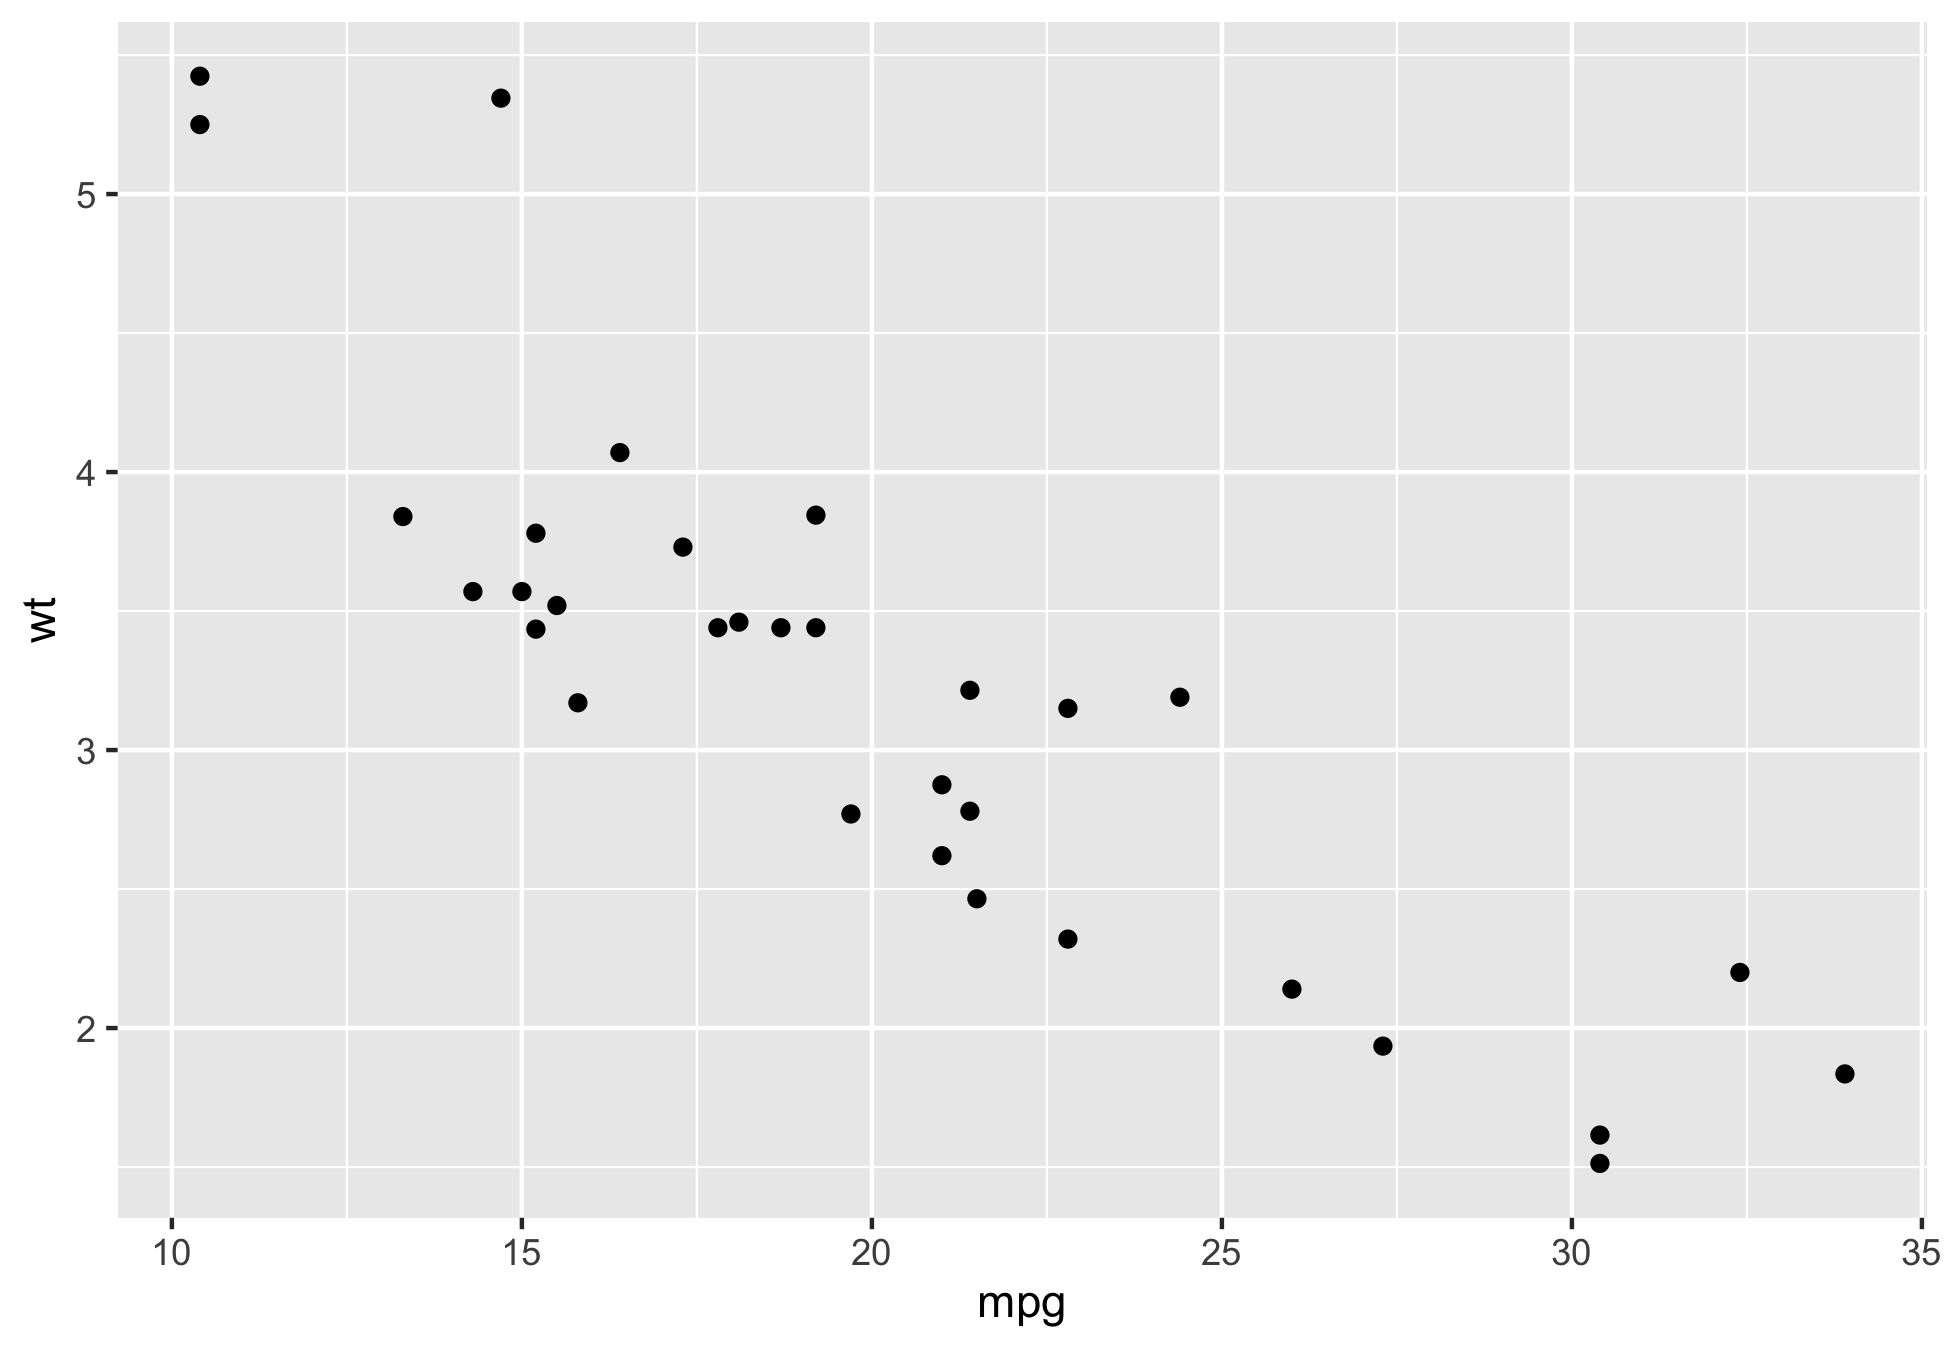
\includegraphics[width=0.7\linewidth]{figurasR/capi05mtcars} \end{center}

También se pueden grabar con las funciones \textbf{\texttt{png()}},
\textbf{\texttt{jpeg()}}, \textbf{\texttt{pdf()}}, etc, y
\textbf{\texttt{dev.off()}}, como se ilustra en los siguientes ejemplos
de código R:

\begin{Shaded}
\begin{Highlighting}[]
\FunctionTok{png}\NormalTok{(}\AttributeTok{file =} \StringTok{"figurasR/capi05myplot.png"}\NormalTok{, }\AttributeTok{bg =} \StringTok{"transparent"}\NormalTok{)}
\FunctionTok{plot}\NormalTok{(}\DecValTok{1}\SpecialCharTok{:}\DecValTok{10}\NormalTok{)}
\FunctionTok{rect}\NormalTok{(}\DecValTok{1}\NormalTok{, }\DecValTok{5}\NormalTok{, }\DecValTok{3}\NormalTok{, }\DecValTok{7}\NormalTok{, }\AttributeTok{col =} \StringTok{"white"}\NormalTok{)}
\FunctionTok{dev.off}\NormalTok{()}
\end{Highlighting}
\end{Shaded}

\begin{Shaded}
\begin{Highlighting}[]
 \CommentTok{\# creará myplot1.jpg y myplot2.jpg}
\FunctionTok{jpeg}\NormalTok{(}\AttributeTok{file =} \StringTok{"figurasR/capi05myplot\%d.jpg"}\NormalTok{)}
\FunctionTok{example}\NormalTok{(rect)}
\FunctionTok{dev.off}\NormalTok{()}
\end{Highlighting}
\end{Shaded}

\hypertarget{incluir-un-gruxe1fico-creado-con-r-sin-leyenda-y-justo-aquuxed}{%
\paragraph{Incluir un gráfico creado con R sin leyenda y justo
aquí}\label{incluir-un-gruxe1fico-creado-con-r-sin-leyenda-y-justo-aquuxed}}

Se demuestra con un ejemplo que usa el paquete ``ggplot2'', en el que
además el gráfico aparece centrado (se ha indicado:
\texttt{fig.align=\textquotesingle{}center\textquotesingle{}}, pero hay
otros valores para esta opción:
\texttt{\textquotesingle{}left\textquotesingle{}},
\texttt{\textquotesingle{}right\textquotesingle{}}. Si no se utiliza
aparece justificada a la izquierda).

\begin{Shaded}
\begin{Highlighting}[]
\InformationTok{\textasciigrave{}\textasciigrave{}\textasciigrave{}\{r echo=FALSE,out.width=\textquotesingle{}80\%\textquotesingle{},fig.align=\textquotesingle{}center\textquotesingle{},fig.pos=\textquotesingle{}H\textquotesingle{}\}}
\InformationTok{library(ggplot2)}
\InformationTok{p = ggplot(mtcars, aes(mpg, wt)) + }
\InformationTok{  geom\_point()}
\InformationTok{p  }
\InformationTok{\textasciigrave{}\textasciigrave{}\textasciigrave{}}
\end{Highlighting}
\end{Shaded}

\begin{center}\includegraphics[width=0.8\linewidth]{figurasR/unnamed-chunk-28-1} \end{center}

\hypertarget{incluir-un-gruxe1fico-creado-con-r-con-leyenda-y-situado-en-la-parte-superior}{%
\paragraph{Incluir un gráfico creado con R con leyenda y situado en la
parte
superior}\label{incluir-un-gruxe1fico-creado-con-r-con-leyenda-y-situado-en-la-parte-superior}}

El gráfico de la Figura \ref{fig:cap05gg02} es un ejemplo de gráfico
creado con R y aparece con una leyenda explicativa y colocado en la
parte superior de la página.

\begin{Shaded}
\begin{Highlighting}[]
\InformationTok{\textasciigrave{}\textasciigrave{}\textasciigrave{}\{r echo=FALSE,out.width=\textquotesingle{}80\%\textquotesingle{},fig.align=\textquotesingle{}center\textquotesingle{},fig.pos=\textquotesingle{}htbp\textquotesingle{},}
\InformationTok{fig.cap="\textbackslash{}\textbackslash{}label\{fig:cap05gg02\}Gr\textbackslash{}\textbackslash{}\textquotesingle{}afico de L\textbackslash{}\textbackslash{}\textquotesingle{}\{\textbackslash{}\textbackslash{}i\}neas creado }
\InformationTok{         con ggplot2 (fuente: elaboraci\textbackslash{}\textbackslash{}\textquotesingle{}on propia)"\}}
\InformationTok{library(ggplot2)}
\InformationTok{ggplot(mtcars, aes(mpg, wt)) + }
\InformationTok{  geom\_line(col="blue")}
\InformationTok{\textasciigrave{}\textasciigrave{}\textasciigrave{}}
\end{Highlighting}
\end{Shaded}

\begin{figure}[htbp]

{\centering \includegraphics[width=0.8\linewidth]{figurasR/unnamed-chunk-29-1} 

}

\caption{\label{fig:cap05gg02}Gr\'afico de L\'{\i}neas creado con ggplot2 (fuente: elaboraci\'on propia)}\label{fig:unnamed-chunk-29}
\end{figure}

\hypertarget{varios-gruxe1ficos-creados-con-r-con-varias-leyendas}{%
\paragraph{Varios gráficos creados con R con varias
leyendas}\label{varios-gruxe1ficos-creados-con-r-con-varias-leyendas}}

Con el siguiente código se pueden presentar dos gráficos en una única
figura y además se puede colocar una leyenda explicativa a cada gráfico
(obtenido en:
\href{https://stackoverflow.com/questions/53850299/how-to-get-a-newline-in-a-figure-caption-in-rmarkdown-bookdown-pdfdocument2}{stackoverflow}).

\textbf{Observe} que no se ha usado \textbf{label} en \texttt{fig.cap},
el identificador se ha construido del identificador del chunk:
``plot-cars'' al que se le ha añadido como prefijo: ``fig:'', quedando
el identificador para usar con \textbf{ref}: ``fig:plot-cars''. A las
subfiguras se les ha añadido números consecutivos.

\begin{Shaded}
\begin{Highlighting}[]

\NormalTok{Vea la Figura \textbackslash{}ref\{fig:plot{-}cars\}, la cual contiene la Figura }
\NormalTok{\textbackslash{}ref\{fig:plot{-}cars{-}1\} y la Figura \textbackslash{}ref\{fig:plot{-}cars{-}2\}.}

\InformationTok{\textasciigrave{}\textasciigrave{}\textasciigrave{}\{r plot{-}cars, fig.height = 3, fig.width = 4,out.width=\textquotesingle{}49\%\textquotesingle{}, }
\InformationTok{fig.cap="Dos gr\textbackslash{}\textbackslash{}\textquotesingle{}aficos", fig.subcap = c("Regresi\textbackslash{}\textbackslash{}\textquotesingle{}on", }
\InformationTok{"Gr\textbackslash{}\textbackslash{}\textquotesingle{}afico sobre cars"),fig.pos="htbp"\}}
\InformationTok{plot(mpg \textasciitilde{} wt, data = mtcars)}
\InformationTok{plot(cars)}
\InformationTok{\textasciigrave{}\textasciigrave{}\textasciigrave{}}
\end{Highlighting}
\end{Shaded}

Vea la Figura \ref{fig:plot-cars}, la cual contiene la Figura
\ref{fig:plot-cars-1} y la Figura \ref{fig:plot-cars-2}.

\begin{Shaded}
\begin{Highlighting}[]
\FunctionTok{plot}\NormalTok{(mpg }\SpecialCharTok{\textasciitilde{}}\NormalTok{ wt, }\AttributeTok{data =}\NormalTok{ mtcars)}
\FunctionTok{plot}\NormalTok{(cars)}
\end{Highlighting}
\end{Shaded}

\begin{figure}[htbp]

{\centering \subfloat[Regresi\'on\label{fig:plot-cars-1}]{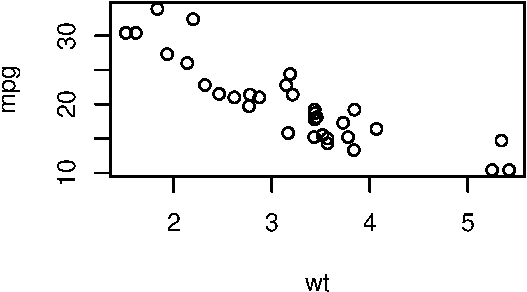
\includegraphics[width=0.49\linewidth]{figurasR/plot-cars-1} }\subfloat[Gr\'afico sobre cars\label{fig:plot-cars-2}]{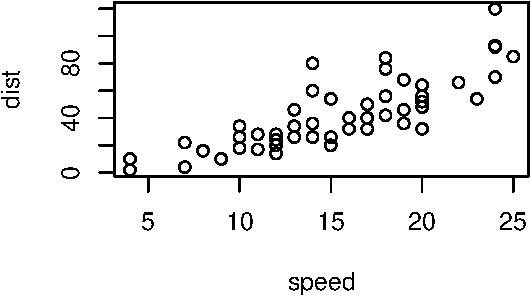
\includegraphics[width=0.49\linewidth]{figurasR/plot-cars-2} }

}

\caption{Dos gr\'aficos}\label{fig:plot-cars}
\end{figure}

Otro ejemplo en el que solamente se usa una leyenda para los dos
gráficos (también se modifican los márgenes). Importante el uso de la
opción de chunk: \textbf{fig.show=``hold''}.

\begin{Shaded}
\begin{Highlighting}[]
\InformationTok{\textasciigrave{}\textasciigrave{}\textasciigrave{}\{r out.width=\textquotesingle{}45\%\textquotesingle{},fig.show="hold",}
\InformationTok{        fig.cap="Dos gr\textbackslash{}\textbackslash{}\textquotesingle{}aficos R cara a cara",fig.pos="htbp"\}}
\InformationTok{par(mar = c(4, 4, 0.1, 0.1))}
\InformationTok{plot(pressure, pch = 19, type = "b")}
\InformationTok{plot(cars, pch = 19)}
\InformationTok{\textasciigrave{}\textasciigrave{}\textasciigrave{}}
\end{Highlighting}
\end{Shaded}

Produce la Figura \ref{fig:fig2}.

\begin{Shaded}
\begin{Highlighting}[]
\FunctionTok{par}\NormalTok{(}\AttributeTok{mar =} \FunctionTok{c}\NormalTok{(}\DecValTok{4}\NormalTok{, }\DecValTok{4}\NormalTok{, }\FloatTok{0.1}\NormalTok{, }\FloatTok{0.1}\NormalTok{))}
\FunctionTok{plot}\NormalTok{(pressure, }\AttributeTok{pch =} \DecValTok{19}\NormalTok{, }\AttributeTok{type =} \StringTok{"b"}\NormalTok{)}
\FunctionTok{plot}\NormalTok{(cars, }\AttributeTok{pch =} \DecValTok{19}\NormalTok{)}
\end{Highlighting}
\end{Shaded}

\begin{figure}[htbp]

{\centering 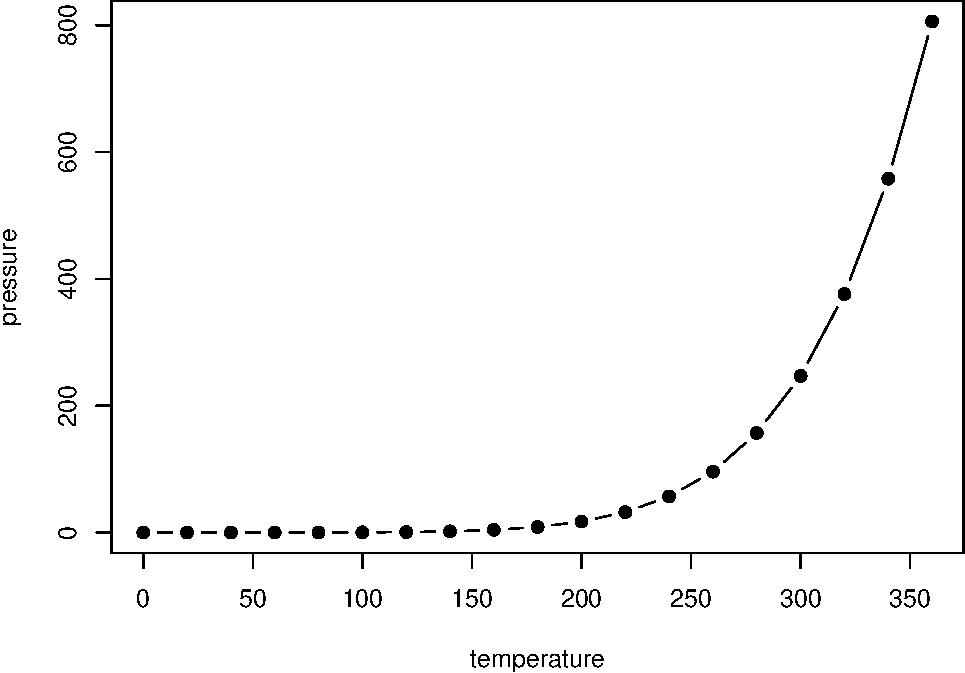
\includegraphics[width=0.45\linewidth]{figurasR/fig2-1} 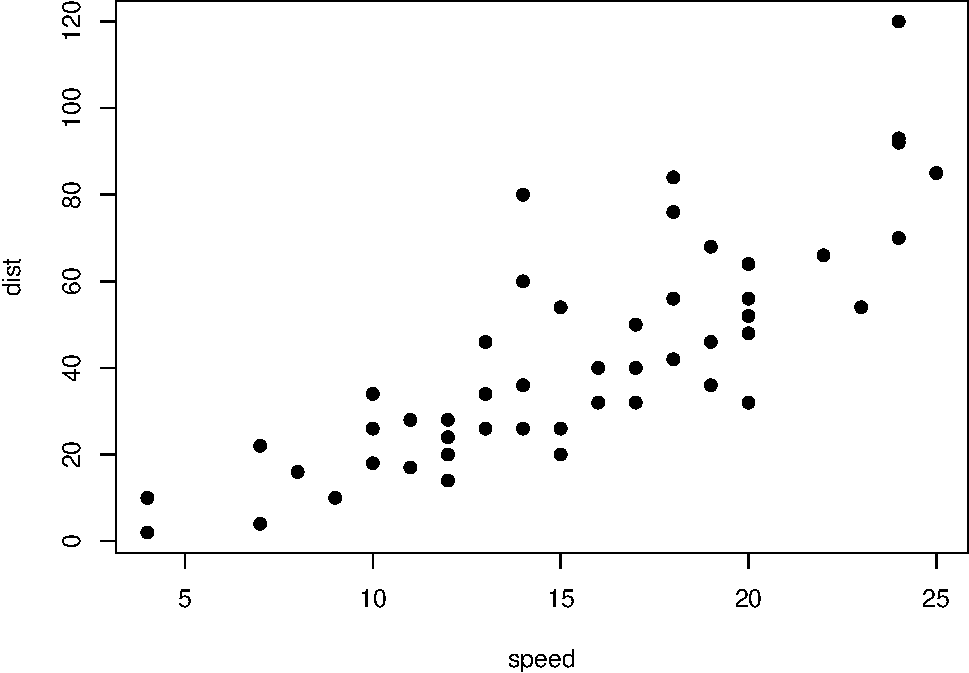
\includegraphics[width=0.45\linewidth]{figurasR/fig2-2} 

}

\caption{Dos gr\'aficos R cara a cara}\label{fig:fig2}
\end{figure}

\hypertarget{cuxf3mo-incluir-una-tabla-o-cuadro-con-informaciuxf3n}{%
\subsection{Cómo incluir una tabla o cuadro con
información}\label{cuxf3mo-incluir-una-tabla-o-cuadro-con-informaciuxf3n}}

Para profundizar en el tema de la presentación de tablas de información
se recomienda visitar la siguiente url:
\href{http://destio.us.es/calvo/post/como-crear-tablas-de-informacion-en-r-markdown/}{Cómo
Crear tablas de información en R Markdown}.

\hypertarget{incluir-una-tabla-con-leyenda}{%
\subsubsection{Incluir una tabla con
leyenda}\label{incluir-una-tabla-con-leyenda}}

La presentación de las primeras 10 filas de un data.frame de R, por
ejemplo, el dataset \texttt{iris}, puede hacerse del siguiente modo:

\begin{Shaded}
\begin{Highlighting}[]
\FunctionTok{head}\NormalTok{(iris,}\DecValTok{10}\NormalTok{)}
\end{Highlighting}
\end{Shaded}

\begin{verbatim}
##    Sepal.Length Sepal.Width Petal.Length Petal.Width Species
## 1           5.1         3.5          1.4         0.2  setosa
## 2           4.9         3.0          1.4         0.2  setosa
## 3           4.7         3.2          1.3         0.2  setosa
## 4           4.6         3.1          1.5         0.2  setosa
## 5           5.0         3.6          1.4         0.2  setosa
## 6           5.4         3.9          1.7         0.4  setosa
## 7           4.6         3.4          1.4         0.3  setosa
## 8           5.0         3.4          1.5         0.2  setosa
## 9           4.4         2.9          1.4         0.2  setosa
## 10          4.9         3.1          1.5         0.1  setosa
\end{verbatim}

Pero para mejorar la presentación se pueden utilizar paquetes R
especializados, como:
\href{https://cran.r-project.org/web/packages/knitr/index.html}{knitr},
\href{https://cran.r-project.org/web/packages/kableExtra/index.html}{kableExtra},
\href{https://cran.r-project.org/web/packages/huxtable/}{huxtable}
(trata aspectos muy avanzados), etc. El siguiente ejemplo ilustra el uso
de ``kableExtra''. Se comentan algunas de las opciones usadas:

\begin{itemize}
\tightlist
\item
  \textbf{\texttt{"hold\_position"}}: usa el posicionamiento como en las
  figuras \textbf{``h''}.
\item
  \textbf{\texttt{position="center"}}: presenta la tabla centrada.
\item
  \textbf{\texttt{"striped"}}: alterna el color de las filas.
\item
  \textbf{\texttt{caption="\textbackslash{}\textbackslash{}label\{\}Explicación..."}}:
  Añade una leyenda que explique el contenido de la tabla junto a un
  identificador para hacer referencia a ella con
  \textbf{\texttt{\textbackslash{}ref\{\}}}.
\end{itemize}

\begin{Shaded}
\begin{Highlighting}[]
\InformationTok{\textasciigrave{}\textasciigrave{}\textasciigrave{}\{r\}}
\InformationTok{library(knitr)}
\InformationTok{library(kableExtra) }
\InformationTok{head(iris,10) \%\textgreater{}\%}
\InformationTok{ kable(booktabs = TRUE,format = "latex",}
\InformationTok{  caption = "\textbackslash{}\textbackslash{}label\{tabla02\}Leyenda explicativa de la segunda tabla") \%\textgreater{}\%}
\InformationTok{ kable\_styling(}
\InformationTok{  latex\_options = c("striped", "condensed","hold\_position"), }
\InformationTok{  position = "center",full\_width = FALSE)}
\InformationTok{\textasciigrave{}\textasciigrave{}\textasciigrave{}}
\end{Highlighting}
\end{Shaded}

Produce el siguiente resultado:

\begin{Shaded}
\begin{Highlighting}[]
\FunctionTok{library}\NormalTok{(knitr)}
\FunctionTok{library}\NormalTok{(kableExtra) }
\FunctionTok{head}\NormalTok{(iris,}\DecValTok{10}\NormalTok{) }\SpecialCharTok{\%\textgreater{}\%}
  \FunctionTok{kable}\NormalTok{(}\AttributeTok{booktabs =} \ConstantTok{TRUE}\NormalTok{,}\AttributeTok{format =} \StringTok{"latex"}\NormalTok{,}
    \AttributeTok{caption =} \StringTok{"}\SpecialCharTok{\textbackslash{}\textbackslash{}}\StringTok{label\{tabla02\}Leyenda explicativa de la segunda tabla"}\NormalTok{) }\SpecialCharTok{\%\textgreater{}\%}
  \FunctionTok{kable\_styling}\NormalTok{(}
    \AttributeTok{latex\_options =} \FunctionTok{c}\NormalTok{(}\StringTok{"striped"}\NormalTok{, }\StringTok{"condensed"}\NormalTok{,}\StringTok{"hold\_position"}\NormalTok{), }
    \AttributeTok{position =} \StringTok{"center"}\NormalTok{,}\AttributeTok{full\_width =} \ConstantTok{FALSE}\NormalTok{)}
\end{Highlighting}
\end{Shaded}

\begin{table}[!h]

\caption{\label{tab:unnamed-chunk-31}\label{tabla02}Leyenda explicativa de la segunda tabla}
\centering
\begin{tabular}[t]{rrrrl}
\toprule
Sepal.Length & Sepal.Width & Petal.Length & Petal.Width & Species\\
\midrule
\cellcolor{gray!6}{5.1} & \cellcolor{gray!6}{3.5} & \cellcolor{gray!6}{1.4} & \cellcolor{gray!6}{0.2} & \cellcolor{gray!6}{setosa}\\
4.9 & 3.0 & 1.4 & 0.2 & setosa\\
\cellcolor{gray!6}{4.7} & \cellcolor{gray!6}{3.2} & \cellcolor{gray!6}{1.3} & \cellcolor{gray!6}{0.2} & \cellcolor{gray!6}{setosa}\\
4.6 & 3.1 & 1.5 & 0.2 & setosa\\
\cellcolor{gray!6}{5.0} & \cellcolor{gray!6}{3.6} & \cellcolor{gray!6}{1.4} & \cellcolor{gray!6}{0.2} & \cellcolor{gray!6}{setosa}\\
\addlinespace
5.4 & 3.9 & 1.7 & 0.4 & setosa\\
\cellcolor{gray!6}{4.6} & \cellcolor{gray!6}{3.4} & \cellcolor{gray!6}{1.4} & \cellcolor{gray!6}{0.3} & \cellcolor{gray!6}{setosa}\\
5.0 & 3.4 & 1.5 & 0.2 & setosa\\
\cellcolor{gray!6}{4.4} & \cellcolor{gray!6}{2.9} & \cellcolor{gray!6}{1.4} & \cellcolor{gray!6}{0.2} & \cellcolor{gray!6}{setosa}\\
4.9 & 3.1 & 1.5 & 0.1 & setosa\\
\bottomrule
\end{tabular}
\end{table}

\hypertarget{incluir-una-tabla-que-ocupe-varias-puxe1ginas}{%
\subsubsection{Incluir una tabla que ocupe varias
páginas}\label{incluir-una-tabla-que-ocupe-varias-puxe1ginas}}

Para corregir esa situación, la librería ``kableExtra'' nos permite
presentar tablas que ocupen varias páginas utilizando los siguientes
argumentos, como puede comprobarse en el ejemplo que se muestra:

\begin{itemize}
\item
  Se ha añadido a \textbf{latex\_options} la opción:
  \textbf{repeat\_header}.
\item
  Se ha indicado el texto que aparecerá antes de pasar a la siguiente
  página:
  \textbf{\texttt{repeat\_header\_continued="contin\textbackslash{}\textbackslash{}\textquotesingle{}ua\ en\ la\ siguiente\ p\textbackslash{}\textbackslash{}\textquotesingle{}agina"}}.
\item
  Se ha indicado también el texto que aparecerá antes de escribir
  información de la tabla en la siguiente página:
  \textbf{\texttt{repeat\_header\_text\ =\ "continuaci\textbackslash{}\textbackslash{}\textquotesingle{}on"}}.
\end{itemize}

El siguiente código:

\begin{Shaded}
\begin{Highlighting}[]
\InformationTok{\textasciigrave{}\textasciigrave{}\textasciigrave{}\{r\}}
\InformationTok{library(kableExtra) }
\InformationTok{iris[1:50,] \%\textgreater{}\% }
\InformationTok{  kable(booktabs = TRUE,format = "latex",digits = 1, longtable=TRUE) \%\textgreater{}\%}
\InformationTok{  kable\_styling(}
\InformationTok{   latex\_options = c("striped", "condensed","repeat\_header"), }
\InformationTok{   position = "center",full\_width = FALSE,}
\InformationTok{   repeat\_header\_text = "continuaci\textbackslash{}\textbackslash{}\textquotesingle{}on", }
\InformationTok{   repeat\_header\_continued="contin\textbackslash{}\textbackslash{}\textquotesingle{}ua en la siguiente p\textbackslash{}\textbackslash{}\textquotesingle{}agina"}
\InformationTok{  )}
\InformationTok{\textasciigrave{}\textasciigrave{}\textasciigrave{}}
\end{Highlighting}
\end{Shaded}

Produce el siguiente resultado:

\begin{Shaded}
\begin{Highlighting}[]
\FunctionTok{library}\NormalTok{(kableExtra) }
\NormalTok{iris[}\DecValTok{1}\SpecialCharTok{:}\DecValTok{50}\NormalTok{,] }\SpecialCharTok{\%\textgreater{}\%} 
  \FunctionTok{kable}\NormalTok{(}\AttributeTok{booktabs =} \ConstantTok{TRUE}\NormalTok{,}\AttributeTok{format =} \StringTok{"latex"}\NormalTok{,}\AttributeTok{digits =} \DecValTok{1}\NormalTok{, }\AttributeTok{longtable=}\ConstantTok{TRUE}\NormalTok{) }\SpecialCharTok{\%\textgreater{}\%}
  \FunctionTok{kable\_styling}\NormalTok{(}
   \AttributeTok{latex\_options =} \FunctionTok{c}\NormalTok{(}\StringTok{"striped"}\NormalTok{, }\StringTok{"condensed"}\NormalTok{,}\StringTok{"repeat\_header"}\NormalTok{), }
   \AttributeTok{position =} \StringTok{"center"}\NormalTok{,}\AttributeTok{full\_width =} \ConstantTok{FALSE}\NormalTok{,}
   \AttributeTok{repeat\_header\_text =} \StringTok{"continuaci}\SpecialCharTok{\textbackslash{}\textbackslash{}}\StringTok{\textquotesingle{}on"}\NormalTok{, }
   \AttributeTok{repeat\_header\_continued=}\StringTok{"contin}\SpecialCharTok{\textbackslash{}\textbackslash{}}\StringTok{\textquotesingle{}ua en la siguiente p}\SpecialCharTok{\textbackslash{}\textbackslash{}}\StringTok{\textquotesingle{}agina"}
\NormalTok{  )}
\end{Highlighting}
\end{Shaded}

\begin{longtable}{rrrrl}
\toprule
Sepal.Length & Sepal.Width & Petal.Length & Petal.Width & Species\\
\midrule
\endfirsthead
\multicolumn{5}{@{}l}{continuaci\'on}\\
\toprule
Sepal.Length & Sepal.Width & Petal.Length & Petal.Width & Species\\
\midrule
\endhead
\midrule
\multicolumn{5}{r@{}}{contin\'ua en la siguiente p\'agina}\
\endfoot
\bottomrule
\endlastfoot
\cellcolor{gray!6}{5.1} & \cellcolor{gray!6}{3.5} & \cellcolor{gray!6}{1.4} & \cellcolor{gray!6}{0.2} & \cellcolor{gray!6}{setosa}\\
4.9 & 3.0 & 1.4 & 0.2 & setosa\\
\cellcolor{gray!6}{4.7} & \cellcolor{gray!6}{3.2} & \cellcolor{gray!6}{1.3} & \cellcolor{gray!6}{0.2} & \cellcolor{gray!6}{setosa}\\
4.6 & 3.1 & 1.5 & 0.2 & setosa\\
\cellcolor{gray!6}{5.0} & \cellcolor{gray!6}{3.6} & \cellcolor{gray!6}{1.4} & \cellcolor{gray!6}{0.2} & \cellcolor{gray!6}{setosa}\\
\addlinespace
5.4 & 3.9 & 1.7 & 0.4 & setosa\\
\cellcolor{gray!6}{4.6} & \cellcolor{gray!6}{3.4} & \cellcolor{gray!6}{1.4} & \cellcolor{gray!6}{0.3} & \cellcolor{gray!6}{setosa}\\
5.0 & 3.4 & 1.5 & 0.2 & setosa\\
\cellcolor{gray!6}{4.4} & \cellcolor{gray!6}{2.9} & \cellcolor{gray!6}{1.4} & \cellcolor{gray!6}{0.2} & \cellcolor{gray!6}{setosa}\\
4.9 & 3.1 & 1.5 & 0.1 & setosa\\
\addlinespace
\cellcolor{gray!6}{5.4} & \cellcolor{gray!6}{3.7} & \cellcolor{gray!6}{1.5} & \cellcolor{gray!6}{0.2} & \cellcolor{gray!6}{setosa}\\
4.8 & 3.4 & 1.6 & 0.2 & setosa\\
\cellcolor{gray!6}{4.8} & \cellcolor{gray!6}{3.0} & \cellcolor{gray!6}{1.4} & \cellcolor{gray!6}{0.1} & \cellcolor{gray!6}{setosa}\\
4.3 & 3.0 & 1.1 & 0.1 & setosa\\
\cellcolor{gray!6}{5.8} & \cellcolor{gray!6}{4.0} & \cellcolor{gray!6}{1.2} & \cellcolor{gray!6}{0.2} & \cellcolor{gray!6}{setosa}\\
\addlinespace
5.7 & 4.4 & 1.5 & 0.4 & setosa\\
\cellcolor{gray!6}{5.4} & \cellcolor{gray!6}{3.9} & \cellcolor{gray!6}{1.3} & \cellcolor{gray!6}{0.4} & \cellcolor{gray!6}{setosa}\\
5.1 & 3.5 & 1.4 & 0.3 & setosa\\
\cellcolor{gray!6}{5.7} & \cellcolor{gray!6}{3.8} & \cellcolor{gray!6}{1.7} & \cellcolor{gray!6}{0.3} & \cellcolor{gray!6}{setosa}\\
5.1 & 3.8 & 1.5 & 0.3 & setosa\\
\addlinespace
\cellcolor{gray!6}{5.4} & \cellcolor{gray!6}{3.4} & \cellcolor{gray!6}{1.7} & \cellcolor{gray!6}{0.2} & \cellcolor{gray!6}{setosa}\\
5.1 & 3.7 & 1.5 & 0.4 & setosa\\
\cellcolor{gray!6}{4.6} & \cellcolor{gray!6}{3.6} & \cellcolor{gray!6}{1.0} & \cellcolor{gray!6}{0.2} & \cellcolor{gray!6}{setosa}\\
5.1 & 3.3 & 1.7 & 0.5 & setosa\\
\cellcolor{gray!6}{4.8} & \cellcolor{gray!6}{3.4} & \cellcolor{gray!6}{1.9} & \cellcolor{gray!6}{0.2} & \cellcolor{gray!6}{setosa}\\
\addlinespace
5.0 & 3.0 & 1.6 & 0.2 & setosa\\
\cellcolor{gray!6}{5.0} & \cellcolor{gray!6}{3.4} & \cellcolor{gray!6}{1.6} & \cellcolor{gray!6}{0.4} & \cellcolor{gray!6}{setosa}\\
5.2 & 3.5 & 1.5 & 0.2 & setosa\\
\cellcolor{gray!6}{5.2} & \cellcolor{gray!6}{3.4} & \cellcolor{gray!6}{1.4} & \cellcolor{gray!6}{0.2} & \cellcolor{gray!6}{setosa}\\
4.7 & 3.2 & 1.6 & 0.2 & setosa\\
\addlinespace
\cellcolor{gray!6}{4.8} & \cellcolor{gray!6}{3.1} & \cellcolor{gray!6}{1.6} & \cellcolor{gray!6}{0.2} & \cellcolor{gray!6}{setosa}\\
5.4 & 3.4 & 1.5 & 0.4 & setosa\\
\cellcolor{gray!6}{5.2} & \cellcolor{gray!6}{4.1} & \cellcolor{gray!6}{1.5} & \cellcolor{gray!6}{0.1} & \cellcolor{gray!6}{setosa}\\
5.5 & 4.2 & 1.4 & 0.2 & setosa\\
\cellcolor{gray!6}{4.9} & \cellcolor{gray!6}{3.1} & \cellcolor{gray!6}{1.5} & \cellcolor{gray!6}{0.2} & \cellcolor{gray!6}{setosa}\\
\addlinespace
5.0 & 3.2 & 1.2 & 0.2 & setosa\\
\cellcolor{gray!6}{5.5} & \cellcolor{gray!6}{3.5} & \cellcolor{gray!6}{1.3} & \cellcolor{gray!6}{0.2} & \cellcolor{gray!6}{setosa}\\
4.9 & 3.6 & 1.4 & 0.1 & setosa\\
\cellcolor{gray!6}{4.4} & \cellcolor{gray!6}{3.0} & \cellcolor{gray!6}{1.3} & \cellcolor{gray!6}{0.2} & \cellcolor{gray!6}{setosa}\\
5.1 & 3.4 & 1.5 & 0.2 & setosa\\
\addlinespace
\cellcolor{gray!6}{5.0} & \cellcolor{gray!6}{3.5} & \cellcolor{gray!6}{1.3} & \cellcolor{gray!6}{0.3} & \cellcolor{gray!6}{setosa}\\
4.5 & 2.3 & 1.3 & 0.3 & setosa\\
\cellcolor{gray!6}{4.4} & \cellcolor{gray!6}{3.2} & \cellcolor{gray!6}{1.3} & \cellcolor{gray!6}{0.2} & \cellcolor{gray!6}{setosa}\\
5.0 & 3.5 & 1.6 & 0.6 & setosa\\
\cellcolor{gray!6}{5.1} & \cellcolor{gray!6}{3.8} & \cellcolor{gray!6}{1.9} & \cellcolor{gray!6}{0.4} & \cellcolor{gray!6}{setosa}\\
\addlinespace
4.8 & 3.0 & 1.4 & 0.3 & setosa\\
\cellcolor{gray!6}{5.1} & \cellcolor{gray!6}{3.8} & \cellcolor{gray!6}{1.6} & \cellcolor{gray!6}{0.2} & \cellcolor{gray!6}{setosa}\\
4.6 & 3.2 & 1.4 & 0.2 & setosa\\
\cellcolor{gray!6}{5.3} & \cellcolor{gray!6}{3.7} & \cellcolor{gray!6}{1.5} & \cellcolor{gray!6}{0.2} & \cellcolor{gray!6}{setosa}\\
5.0 & 3.3 & 1.4 & 0.2 & setosa\\*
\end{longtable}

\& 0.2 \& setosa\textbackslash* \textbackslash end\{longtable\}

\hypertarget{incluir-una-tabla-con-aspecto-de-lista-diccionario}{%
\subsubsection{Incluir una tabla con aspecto de
lista-diccionario}\label{incluir-una-tabla-con-aspecto-de-lista-diccionario}}

El siguiente código:

\begin{Shaded}
\begin{Highlighting}[]
\InformationTok{\textasciigrave{}\textasciigrave{}\textasciigrave{}\{r\}}
\InformationTok{text\_tbl \textless{}{-} data.frame(}
\InformationTok{  Items = c("Item 1", "Item 2", "Item 3"), }
\InformationTok{  Features = c(}
\InformationTok{    "Lorem ipsum dolor sit amet, consectetur adipiscing elit.}
\InformationTok{    Proin vehicula tempor ex. Morbi malesuada sagittis turpis,}
\InformationTok{    at venenatis nisl luctus a. ",}
\InformationTok{    "In eu urna at magna luctus rhoncus quis in nisl. Fusce in velit}
\InformationTok{    varius, posuere risus et, cursus augue. Duis eleifend aliquam ante,}
\InformationTok{    a aliquet ex tincidunt in. ",}
\InformationTok{    "Vivamus venenatis egestas eros ut tempus. Vivamus id est nisi.}
\InformationTok{    Aliquam molestie erat et sollicitudin venenatis. In ac lacus at}
\InformationTok{    velit scelerisque mattis. "}
\InformationTok{    ) }
\InformationTok{  )}

\InformationTok{kable(text\_tbl, "latex", booktabs = T) \%\textgreater{}\% }
\InformationTok{  kable\_styling(full\_width = F) \%\textgreater{}\% }
\InformationTok{  column\_spec(1, bold = T, color = "red") \%\textgreater{}\% }
\InformationTok{  column\_spec(2, width = "30em")}
\InformationTok{\textasciigrave{}\textasciigrave{}\textasciigrave{}}
\end{Highlighting}
\end{Shaded}

Produce el siguiente resultado:

\begin{Shaded}
\begin{Highlighting}[]
\NormalTok{text\_tbl }\OtherTok{\textless{}{-}} \FunctionTok{data.frame}\NormalTok{(}
  \AttributeTok{Items =} \FunctionTok{c}\NormalTok{(}\StringTok{"Item 1"}\NormalTok{, }\StringTok{"Item 2"}\NormalTok{, }\StringTok{"Item 3"}\NormalTok{), }
  \AttributeTok{Features =} \FunctionTok{c}\NormalTok{(}
    \StringTok{"Lorem ipsum dolor sit amet, consectetur adipiscing elit.}
\StringTok{    Proin vehicula tempor ex. Morbi malesuada sagittis turpis,}
\StringTok{    at venenatis nisl luctus a. "}\NormalTok{,}
    \StringTok{"In eu urna at magna luctus rhoncus quis in nisl. Fusce in velit}
\StringTok{    varius, posuere risus et, cursus augue. Duis eleifend aliquam ante,}
\StringTok{    a aliquet ex tincidunt in. "}\NormalTok{,}
    \StringTok{"Vivamus venenatis egestas eros ut tempus. Vivamus id est nisi.}
\StringTok{    Aliquam molestie erat et sollicitudin venenatis. In ac lacus at}
\StringTok{    velit scelerisque mattis. "}
\NormalTok{    ) }
\NormalTok{  )}

\FunctionTok{kable}\NormalTok{(text\_tbl, }\StringTok{"latex"}\NormalTok{, }\AttributeTok{booktabs =}\NormalTok{ T) }\SpecialCharTok{\%\textgreater{}\%} 
  \FunctionTok{kable\_styling}\NormalTok{(}\AttributeTok{full\_width =}\NormalTok{ F) }\SpecialCharTok{\%\textgreater{}\%} 
  \FunctionTok{column\_spec}\NormalTok{(}\DecValTok{1}\NormalTok{, }\AttributeTok{bold =}\NormalTok{ T, }\AttributeTok{color =} \StringTok{"red"}\NormalTok{) }\SpecialCharTok{\%\textgreater{}\%} 
  \FunctionTok{column\_spec}\NormalTok{(}\DecValTok{2}\NormalTok{, }\AttributeTok{width =} \StringTok{"30em"}\NormalTok{)}
\end{Highlighting}
\end{Shaded}

\begin{table}
\centering
\begin{tabular}{>{}l>{\raggedright\arraybackslash}p{30em}}
\toprule
Items & Features\\
\midrule
Item 1 & Lorem ipsum dolor sit amet, consectetur adipiscing elit.
    Proin vehicula tempor ex. Morbi malesuada sagittis turpis,
\textcolor{red}{\textbf{    at venenatis nisl luctus a.}}\\
Item 2 & In eu urna at magna luctus rhoncus quis in nisl. Fusce in velit
    varius, posuere risus et, cursus augue. Duis eleifend aliquam ante,
\textcolor{red}{\textbf{    a aliquet ex tincidunt in.}}\\
Item 3 & Vivamus venenatis egestas eros ut tempus. Vivamus id est nisi.
    Aliquam molestie erat et sollicitudin venenatis. In ac lacus at
\textcolor{red}{\textbf{    velit scelerisque mattis.}}\\
\bottomrule
\end{tabular}
\end{table}

\hypertarget{incluir-una-tabla-con-notas-a-pie-de-tabla}{%
\subsubsection{Incluir una tabla con notas a pie de
tabla}\label{incluir-una-tabla-con-notas-a-pie-de-tabla}}

El siguiente código

\begin{Shaded}
\begin{Highlighting}[]
\InformationTok{\textasciigrave{}\textasciigrave{}\textasciigrave{}\{r\}}
\InformationTok{library(kableExtra)}
\InformationTok{dt \textless{}{-} mtcars[1:5, 1:6]}

\InformationTok{kable(dt, "latex", align = "cccrcc", booktabs = T) \%\textgreater{}\%}
\InformationTok{    kable\_styling(position = "left") \%\textgreater{}\% }
\InformationTok{    footnote(general = "Elaboración propia. ",}
\InformationTok{             number = c("Footnote 1; ", "Footnote 2; "),}
\InformationTok{             alphabet = c("Footnote A; ", "Footnote B; "),}
\InformationTok{             symbol = c("Footnote Symbol 1; ", "Footnote Symbol 2"), }
\InformationTok{             general\_title = "Fuente: ", }
\InformationTok{             number\_title = "Type I: ", }
\InformationTok{             alphabet\_title = "Type II: ", }
\InformationTok{             symbol\_title = "Type III: ", }
\InformationTok{             footnote\_as\_chunk = T, }
\InformationTok{             title\_format = c("italic", "underline") )}
\InformationTok{\textasciigrave{}\textasciigrave{}\textasciigrave{}}
\end{Highlighting}
\end{Shaded}

Produce la siguiente salida (la tabla está justificada a la izquierda
\textbf{\texttt{position\ =\ "left"}}):

\begin{Shaded}
\begin{Highlighting}[]
\FunctionTok{library}\NormalTok{(kableExtra)}
\NormalTok{dt }\OtherTok{\textless{}{-}}\NormalTok{ mtcars[}\DecValTok{1}\SpecialCharTok{:}\DecValTok{5}\NormalTok{, }\DecValTok{1}\SpecialCharTok{:}\DecValTok{6}\NormalTok{]}

\FunctionTok{kable}\NormalTok{(dt, }\StringTok{"latex"}\NormalTok{, }\AttributeTok{align =} \StringTok{"cccrcc"}\NormalTok{, }\AttributeTok{booktabs =}\NormalTok{ T) }\SpecialCharTok{\%\textgreater{}\%}
    \FunctionTok{kable\_styling}\NormalTok{(}\AttributeTok{position =} \StringTok{"left"}\NormalTok{) }\SpecialCharTok{\%\textgreater{}\%} 
    \FunctionTok{footnote}\NormalTok{(}\AttributeTok{general =} \StringTok{"Elaboración propia. "}\NormalTok{,}
             \AttributeTok{number =} \FunctionTok{c}\NormalTok{(}\StringTok{"Footnote 1; "}\NormalTok{, }\StringTok{"Footnote 2; "}\NormalTok{),}
             \AttributeTok{alphabet =} \FunctionTok{c}\NormalTok{(}\StringTok{"Footnote A; "}\NormalTok{, }\StringTok{"Footnote B; "}\NormalTok{),}
             \AttributeTok{symbol =} \FunctionTok{c}\NormalTok{(}\StringTok{"Footnote Symbol 1; "}\NormalTok{, }\StringTok{"Footnote Symbol 2"}\NormalTok{), }
             \AttributeTok{general\_title =} \StringTok{"Fuente: "}\NormalTok{, }
             \AttributeTok{number\_title =} \StringTok{"Type I: "}\NormalTok{, }
             \AttributeTok{alphabet\_title =} \StringTok{"Type II: "}\NormalTok{, }
             \AttributeTok{symbol\_title =} \StringTok{"Type III: "}\NormalTok{, }
             \AttributeTok{footnote\_as\_chunk =}\NormalTok{ T, }
             \AttributeTok{title\_format =} \FunctionTok{c}\NormalTok{(}\StringTok{"italic"}\NormalTok{, }\StringTok{"underline"}\NormalTok{) )}
\end{Highlighting}
\end{Shaded}

\begin{tabular}{lcccrcc}
\toprule
  & mpg & cyl & disp & hp & drat & wt\\
\midrule
Mazda RX4 & 21.0 & 6 & 160 & 110 & 3.90 & 2.620\\
Mazda RX4 Wag & 21.0 & 6 & 160 & 110 & 3.90 & 2.875\\
Datsun 710 & 22.8 & 4 & 108 & 93 & 3.85 & 2.320\\
Hornet 4 Drive & 21.4 & 6 & 258 & 110 & 3.08 & 3.215\\
Hornet Sportabout & 18.7 & 8 & 360 & 175 & 3.15 & 3.440\\
\bottomrule
\multicolumn{7}{l}{\rule{0pt}{1em}\underline{\textit{Fuente: }} Elaboración propia. }\\
\multicolumn{7}{l}{\rule{0pt}{1em}\underline{\textit{Type I: }} \textsuperscript{1} Footnote 1;  \textsuperscript{2} Footnote 2; }\\
\multicolumn{7}{l}{\rule{0pt}{1em}\underline{\textit{Type II: }} \textsuperscript{a} Footnote A;  \textsuperscript{b} Footnote B; }\\
\multicolumn{7}{l}{\rule{0pt}{1em}\underline{\textit{Type III: }} \textsuperscript{*} Footnote Symbol 1;  \textsuperscript{\dag} Footnote Symbol 2}\\
\end{tabular}

\hypertarget{presentar-una-tabla-en-modo-apaisado}{%
\subsubsection{Presentar una tabla en modo
apaisado}\label{presentar-una-tabla-en-modo-apaisado}}

Se presentan tres ejemplos de tablas apaisadas.

\begin{enumerate}
\def\labelenumi{\arabic{enumi}.}
\tightlist
\item
  La tabla \ref{tab:apaisada} tiene de especial que se usa la función
  \textbf{\texttt{landscape()}}.
\end{enumerate}

\begin{Shaded}
\begin{Highlighting}[]
\InformationTok{\textasciigrave{}\textasciigrave{}\textasciigrave{}\{r\}}
\InformationTok{text\_tbl \textless{}{-} data.frame(}
\InformationTok{  Items = c("Item 1", "Item 2", "Item 3","Item 4", "Item 5", "Item 6",}
\InformationTok{    "Item 7", "Item 8", "Item 9"), }
\InformationTok{  Features = c(}
\InformationTok{    "Lorem ipsum dolor sit amet, consectetur adipiscing elit.}
\InformationTok{    Proin vehicula tempor ex. Morbi malesuada sagittis turpis,}
\InformationTok{    at venenatis nisl luctus a. ",}
\InformationTok{    "In eu urna at magna luctus rhoncus quis in nisl. Fusce in velit}
\InformationTok{    varius, posuere risus et, cursus augue. Duis eleifend aliquam ante,}
\InformationTok{    a aliquet ex tincidunt in. ",}
\InformationTok{    "Vivamus venenatis egestas eros ut tempus. Vivamus id est nisi.}
\InformationTok{    Aliquam molestie erat et sollicitudin venenatis. In ac lacus at}
\InformationTok{    velit scelerisque mattis. ",}
\InformationTok{    "Lorem ipsum dolor sit amet, consectetur adipiscing elit.}
\InformationTok{    Proin vehicula tempor ex. Morbi malesuada sagittis turpis,}
\InformationTok{    at venenatis nisl luctus a. ",}
\InformationTok{    "In eu urna at magna luctus rhoncus quis in nisl. Fusce in velit}
\InformationTok{    varius, posuere risus et, cursus augue. Duis eleifend aliquam ante,}
\InformationTok{    a aliquet ex tincidunt in. ",}
\InformationTok{    "Vivamus venenatis egestas eros ut tempus. Vivamus id est nisi.}
\InformationTok{    Aliquam molestie erat et sollicitudin venenatis. In ac lacus at}
\InformationTok{    velit scelerisque mattis. ",}
\InformationTok{    "Lorem ipsum dolor sit amet, consectetur adipiscing elit.}
\InformationTok{    Proin vehicula tempor ex. Morbi malesuada sagittis turpis,}
\InformationTok{    at venenatis nisl luctus a. ",}
\InformationTok{    "In eu urna at magna luctus rhoncus quis in nisl. Fusce in velit}
\InformationTok{    varius, posuere risus et, cursus augue. Duis eleifend aliquam ante,}
\InformationTok{    a aliquet ex tincidunt in. ",}
\InformationTok{    "Vivamus venenatis egestas eros ut tempus. Vivamus id est nisi.}
\InformationTok{    Aliquam molestie erat et sollicitudin venenatis. In ac lacus at}
\InformationTok{    velit scelerisque mattis. "}
\InformationTok{    ) }
\InformationTok{  )}
\InformationTok{text\_tbl \%\textgreater{}\%}
\InformationTok{  kable(booktabs = TRUE,caption="\textbackslash{}\textbackslash{}label\{tab:apaisada\}Esta tabla }
\InformationTok{          est\textbackslash{}\textbackslash{}\textquotesingle{}a apaisada y en una p\textbackslash{}\textbackslash{}\textquotesingle{}agina separada") \%\textgreater{}\% }
\InformationTok{      column\_spec(c(1), }
\InformationTok{          width = "2cm") \%\textgreater{}\% }
\InformationTok{      column\_spec(c(2), }
\InformationTok{          width = "10cm") \%\textgreater{}\% }
\InformationTok{      landscape()}
\InformationTok{\textasciigrave{}\textasciigrave{}\textasciigrave{}}
\end{Highlighting}
\end{Shaded}

\begin{enumerate}
\def\labelenumi{\arabic{enumi}.}
\setcounter{enumi}{1}
\item
  La tabla \ref{tab:apaisada2} tiene las siguientes características:

  \begin{itemize}
  \tightlist
  \item
    \texttt{\textbackslash{}hspace\{2cm\}}: desplaza la tabla hacia la
    derecha desde el margen izquierdo-largo.
  \item
    \texttt{skip=50pt}: desplaza verticalmente la tabla hacia abajo.
  \end{itemize}
\end{enumerate}

\begin{Shaded}
\begin{Highlighting}[]

\NormalTok{\textbackslash{}begingroup}
\NormalTok{\textbackslash{}captionsetup\{type=table,skip=50pt\}}
\NormalTok{\textbackslash{}caption\{Es una tabla apaisada ...\} \textbackslash{}label\{tab:apaisada2\}}
\NormalTok{\textbackslash{}hspace\{2cm\}}
\NormalTok{\textbackslash{}Rotatebox\{90\}\{}
\InformationTok{\textasciigrave{}\textasciigrave{}\textasciigrave{}\{r echo=FALSE, warning=FALSE\}}
\InformationTok{library(knitr)}
\InformationTok{library(kableExtra)}
\InformationTok{library(dplyr)}

\InformationTok{text\_tbl \%\textgreater{}\%}
\InformationTok{  kable(booktabs = TRUE) \%\textgreater{}\% }
\InformationTok{      column\_spec(c(1), width = "2cm") \%\textgreater{}\% }
\InformationTok{      column\_spec(c(2), width = "14cm")}

\InformationTok{\textasciigrave{}\textasciigrave{}\textasciigrave{}}
\NormalTok{\}}
\NormalTok{\textbackslash{}endgroup}

\NormalTok{\textbackslash{}newpage}
\end{Highlighting}
\end{Shaded}

\begin{enumerate}
\def\labelenumi{\arabic{enumi}.}
\setcounter{enumi}{2}
\tightlist
\item
  La tabla \ref{tab:sidewaystable} es un ejemplo de uso del entorno
  LaTeX ``sidewaystable'' (en el paquete ``rotating'' incluido) que rota
  la tabla y la leyenda.
\end{enumerate}

\begin{Shaded}
\begin{Highlighting}[]
\NormalTok{text\_tbl }\OtherTok{\textless{}{-}} \FunctionTok{data.frame}\NormalTok{(}
  \AttributeTok{Items =} \FunctionTok{c}\NormalTok{(}\StringTok{"Item 1"}\NormalTok{, }\StringTok{"Item 2"}\NormalTok{, }\StringTok{"Item 3"}\NormalTok{,}\StringTok{"Item 4"}\NormalTok{, }\StringTok{"Item 5"}\NormalTok{, }\StringTok{"Item 6"}\NormalTok{, }
            \StringTok{"Item 7"}\NormalTok{, }\StringTok{"Item 8"}\NormalTok{, }\StringTok{"Item 9"}\NormalTok{), }
  \AttributeTok{Features =} \FunctionTok{c}\NormalTok{(}
    \StringTok{"Lorem ipsum dolor sit amet, consectetur adipiscing elit.}
\StringTok{    Proin vehicula tempor ex. Morbi malesuada sagittis turpis,}
\StringTok{    at venenatis nisl luctus a. "}\NormalTok{,}
    \StringTok{"In eu urna at magna luctus rhoncus quis in nisl. Fusce in velit}
\StringTok{    varius, posuere risus et, cursus augue. Duis eleifend aliquam ante,}
\StringTok{    a aliquet ex tincidunt in. "}\NormalTok{,}
    \StringTok{"Vivamus venenatis egestas eros ut tempus. Vivamus id est nisi.}
\StringTok{    Aliquam molestie erat et sollicitudin venenatis. In ac lacus at}
\StringTok{    velit scelerisque mattis. "}\NormalTok{,}
    \StringTok{"Lorem ipsum dolor sit amet, consectetur adipiscing elit.}
\StringTok{    Proin vehicula tempor ex. Morbi malesuada sagittis turpis,}
\StringTok{    at venenatis nisl luctus a. "}\NormalTok{,}
    \StringTok{"In eu urna at magna luctus rhoncus quis in nisl. Fusce in velit}
\StringTok{    varius, posuere risus et, cursus augue. Duis eleifend aliquam ante,}
\StringTok{    a aliquet ex tincidunt in. "}\NormalTok{,}
    \StringTok{"Vivamus venenatis egestas eros ut tempus. Vivamus id est nisi.}
\StringTok{    Aliquam molestie erat et sollicitudin venenatis. In ac lacus at}
\StringTok{    velit scelerisque mattis. "}\NormalTok{,}
    \StringTok{"Lorem ipsum dolor sit amet, consectetur adipiscing elit.}
\StringTok{    Proin vehicula tempor ex. Morbi malesuada sagittis turpis,}
\StringTok{    at venenatis nisl luctus a. "}\NormalTok{,}
    \StringTok{"In eu urna at magna luctus rhoncus quis in nisl. Fusce in velit}
\StringTok{    varius, posuere risus et, cursus augue. Duis eleifend aliquam ante,}
\StringTok{    a aliquet ex tincidunt in. "}\NormalTok{,}
    \StringTok{"Vivamus venenatis egestas eros ut tempus. Vivamus id est nisi.}
\StringTok{    Aliquam molestie erat et sollicitudin venenatis. In ac lacus at}
\StringTok{    velit scelerisque mattis. "}
\NormalTok{    ) }
\NormalTok{  )}
\NormalTok{text\_tbl }\SpecialCharTok{\%\textgreater{}\%}
  \FunctionTok{kable}\NormalTok{(}\AttributeTok{booktabs =} \ConstantTok{TRUE}\NormalTok{,}\AttributeTok{caption=}\StringTok{"}\SpecialCharTok{\textbackslash{}\textbackslash{}}\StringTok{label\{tab:apaisada\}Esta tabla }
\StringTok{          est}\SpecialCharTok{\textbackslash{}\textbackslash{}}\StringTok{\textquotesingle{}a apaisada y en una p}\SpecialCharTok{\textbackslash{}\textbackslash{}}\StringTok{\textquotesingle{}agina separada"}\NormalTok{) }\SpecialCharTok{\%\textgreater{}\%} 
      \FunctionTok{column\_spec}\NormalTok{(}\FunctionTok{c}\NormalTok{(}\DecValTok{1}\NormalTok{), }
          \AttributeTok{width =} \StringTok{"2cm"}\NormalTok{) }\SpecialCharTok{\%\textgreater{}\%} 
      \FunctionTok{column\_spec}\NormalTok{(}\FunctionTok{c}\NormalTok{(}\DecValTok{2}\NormalTok{), }
          \AttributeTok{width =} \StringTok{"10cm"}\NormalTok{) }\SpecialCharTok{\%\textgreater{}\%} 
      \FunctionTok{landscape}\NormalTok{()}
\end{Highlighting}
\end{Shaded}

\begin{landscape}\begin{table}

\caption{\label{tab:unnamed-chunk-35}\label{tab:apaisada}Esta tabla 
          est\'a apaisada y en una p\'agina separada}
\centering
\begin{tabular}[t]{>{\raggedright\arraybackslash}p{2cm}>{\raggedright\arraybackslash}p{10cm}}
\toprule
Items & Features\\
\midrule
Item 1 & Lorem ipsum dolor sit amet, consectetur adipiscing elit.
    Proin vehicula tempor ex. Morbi malesuada sagittis turpis,
    at venenatis nisl luctus \vphantom{2} a.\\
Item 2 & In eu urna at magna luctus rhoncus quis in nisl. Fusce in velit
    varius, posuere risus et, cursus augue. Duis eleifend aliquam ante,
    a aliquet ex tincidunt \vphantom{2} in.\\
Item 3 & Vivamus venenatis egestas eros ut tempus. Vivamus id est nisi.
    Aliquam molestie erat et sollicitudin venenatis. In ac lacus at
    velit scelerisque \vphantom{2} mattis.\\
Item 4 & Lorem ipsum dolor sit amet, consectetur adipiscing elit.
    Proin vehicula tempor ex. Morbi malesuada sagittis turpis,
    at venenatis nisl luctus \vphantom{1} a.\\
Item 5 & In eu urna at magna luctus rhoncus quis in nisl. Fusce in velit
    varius, posuere risus et, cursus augue. Duis eleifend aliquam ante,
    a aliquet ex tincidunt \vphantom{1} in.\\
\addlinespace
Item 6 & Vivamus venenatis egestas eros ut tempus. Vivamus id est nisi.
    Aliquam molestie erat et sollicitudin venenatis. In ac lacus at
    velit scelerisque \vphantom{1} mattis.\\
Item 7 & Lorem ipsum dolor sit amet, consectetur adipiscing elit.
    Proin vehicula tempor ex. Morbi malesuada sagittis turpis,
    at venenatis nisl luctus a.\\
Item 8 & In eu urna at magna luctus rhoncus quis in nisl. Fusce in velit
    varius, posuere risus et, cursus augue. Duis eleifend aliquam ante,
    a aliquet ex tincidunt in.\\
Item 9 & Vivamus venenatis egestas eros ut tempus. Vivamus id est nisi.
    Aliquam molestie erat et sollicitudin venenatis. In ac lacus at
    velit scelerisque mattis.\\
\bottomrule
\end{tabular}
\end{table}
\end{landscape}

\newpage

\begingroup
\captionsetup{type=table,skip=50pt}
\caption{Es una tabla apaisada ...} \label{tab:apaisada2}
\hspace{2cm}
\Rotatebox{90}{

\begin{tabular}{>{\raggedright\arraybackslash}p{2cm}>{\raggedright\arraybackslash}p{14cm}}
\toprule
Items & Features\\
\midrule
Item 1 & Lorem ipsum dolor sit amet, consectetur adipiscing elit.
    Proin vehicula tempor ex. Morbi malesuada sagittis turpis,
    at venenatis nisl luctus \vphantom{2} a.\\
Item 2 & In eu urna at magna luctus rhoncus quis in nisl. Fusce in velit
    varius, posuere risus et, cursus augue. Duis eleifend aliquam ante,
    a aliquet ex tincidunt \vphantom{2} in.\\
Item 3 & Vivamus venenatis egestas eros ut tempus. Vivamus id est nisi.
    Aliquam molestie erat et sollicitudin venenatis. In ac lacus at
    velit scelerisque \vphantom{2} mattis.\\
Item 4 & Lorem ipsum dolor sit amet, consectetur adipiscing elit.
    Proin vehicula tempor ex. Morbi malesuada sagittis turpis,
    at venenatis nisl luctus \vphantom{1} a.\\
Item 5 & In eu urna at magna luctus rhoncus quis in nisl. Fusce in velit
    varius, posuere risus et, cursus augue. Duis eleifend aliquam ante,
    a aliquet ex tincidunt \vphantom{1} in.\\
\addlinespace
Item 6 & Vivamus venenatis egestas eros ut tempus. Vivamus id est nisi.
    Aliquam molestie erat et sollicitudin venenatis. In ac lacus at
    velit scelerisque \vphantom{1} mattis.\\
Item 7 & Lorem ipsum dolor sit amet, consectetur adipiscing elit.
    Proin vehicula tempor ex. Morbi malesuada sagittis turpis,
    at venenatis nisl luctus a.\\
Item 8 & In eu urna at magna luctus rhoncus quis in nisl. Fusce in velit
    varius, posuere risus et, cursus augue. Duis eleifend aliquam ante,
    a aliquet ex tincidunt in.\\
Item 9 & Vivamus venenatis egestas eros ut tempus. Vivamus id est nisi.
    Aliquam molestie erat et sollicitudin venenatis. In ac lacus at
    velit scelerisque mattis.\\
\bottomrule
\end{tabular}
}
\endgroup

\newpage

\begingroup
\begin{sidewaystable}
\centering
\caption{Es una tabla apaisada ...} \label{tab:sidewaystable}

\begin{tabular}{>{\raggedright\arraybackslash}p{2cm}>{\raggedright\arraybackslash}p{14cm}}
\toprule
Items & Features\\
\midrule
Item 1 & Lorem ipsum dolor sit amet, consectetur adipiscing elit.
    Proin vehicula tempor ex. Morbi malesuada sagittis turpis,
    at venenatis nisl luctus \vphantom{2} a.\\
Item 2 & In eu urna at magna luctus rhoncus quis in nisl. Fusce in velit
    varius, posuere risus et, cursus augue. Duis eleifend aliquam ante,
    a aliquet ex tincidunt \vphantom{2} in.\\
Item 3 & Vivamus venenatis egestas eros ut tempus. Vivamus id est nisi.
    Aliquam molestie erat et sollicitudin venenatis. In ac lacus at
    velit scelerisque \vphantom{2} mattis.\\
Item 4 & Lorem ipsum dolor sit amet, consectetur adipiscing elit.
    Proin vehicula tempor ex. Morbi malesuada sagittis turpis,
    at venenatis nisl luctus \vphantom{1} a.\\
Item 5 & In eu urna at magna luctus rhoncus quis in nisl. Fusce in velit
    varius, posuere risus et, cursus augue. Duis eleifend aliquam ante,
    a aliquet ex tincidunt \vphantom{1} in.\\
\addlinespace
Item 6 & Vivamus venenatis egestas eros ut tempus. Vivamus id est nisi.
    Aliquam molestie erat et sollicitudin venenatis. In ac lacus at
    velit scelerisque \vphantom{1} mattis.\\
Item 7 & Lorem ipsum dolor sit amet, consectetur adipiscing elit.
    Proin vehicula tempor ex. Morbi malesuada sagittis turpis,
    at venenatis nisl luctus a.\\
Item 8 & In eu urna at magna luctus rhoncus quis in nisl. Fusce in velit
    varius, posuere risus et, cursus augue. Duis eleifend aliquam ante,
    a aliquet ex tincidunt in.\\
Item 9 & Vivamus venenatis egestas eros ut tempus. Vivamus id est nisi.
    Aliquam molestie erat et sollicitudin venenatis. In ac lacus at
    velit scelerisque mattis.\\
\bottomrule
\end{tabular}
\end{sidewaystable}
\endgroup

\clearpage

\hypertarget{cambiar-la-etiqueta-tabla}{%
\subsubsection{Cambiar la etiqueta
``Tabla''}\label{cambiar-la-etiqueta-tabla}}

Para que en lugar de ``Tabla'' aparezca ``Cuadro'' (este término es el
que recomienda la RAE), se deberían hacer las siguientes modificaciones
en:

\begin{itemize}
\item
  en el fichero principal ``tfe\_principal.Rmd''

\begin{Shaded}
\begin{Highlighting}[]
\FunctionTok{\textbackslash{}addcontentsline}\NormalTok{\{toc\}\{section\}\{Índice de Tablas\}}
\end{Highlighting}
\end{Shaded}
\item
  Quitar la opción ``es-tabla'' en el fichero
  ``latex/templateMemoriaTFE.tex''

\begin{Shaded}
\begin{Highlighting}[]
\CommentTok{\%\textbackslash{}usepackage[spanish,es{-}nodecimaldot,es{-}noshorthands,es{-}tabla]\{babel\}}
\BuiltInTok{\textbackslash{}usepackage}\NormalTok{[spanish,es{-}nodecimaldot,es{-}noshorthands]\{}\ExtensionTok{babel}\NormalTok{\}}
\end{Highlighting}
\end{Shaded}
\end{itemize}

Más información en la url siguiente:
\href{https://osl.ugr.es/CTAN/macros/latex/contrib/babel-contrib/spanish/spanish.pdf}{Documentación
babel-spanish en CTAN}.

\hypertarget{uso-de-expresiones-matemuxe1ticas}{%
\subsection{Uso de expresiones
matemáticas}\label{uso-de-expresiones-matemuxe1ticas}}

En el siguiente enlace
\href{https://www.overleaf.com/learn/latex/List_of_Greek_letters_and_math_symbols}{overleaf:
alfabeto griego y símbolos matemáticos} puede encontrarse una
recopilación de los comandos LaTeX para representar todo el alfabeto
griego y muchos de los símbolos más usados en expresiones matemáticas.

\hypertarget{algunas-expresiones-matemuxe1ticas}{%
\subsubsection{Algunas expresiones
matemáticas}\label{algunas-expresiones-matemuxe1ticas}}

Las fracciones pueden usarse en el texto, por ejemplo \(\frac{1}{2}\), y
en un estilo matemático centrado como puede verse a continuación:

\[\frac{1}{2}\]

El código utilizado ha sido:

\begin{Shaded}
\begin{Highlighting}[]
\NormalTok{Las fracciones pueden usarse en el texto, por ejemplo }\SpecialCharTok{\textbackslash{}(}\NormalTok{ \textbackslash{}frac\{1\}\{2\} }\SpecialCharTok{\textbackslash{})}\NormalTok{, }
\NormalTok{y en un estilo matemático centrado como puede verse a continuación:}
 
\SpecialCharTok{\textbackslash{}[}\NormalTok{\textbackslash{}frac\{1\}\{2\}}\SpecialCharTok{\textbackslash{}]}
\end{Highlighting}
\end{Shaded}

\begin{itemize}
\item
  Como puede verse
  \textbf{\texttt{\textbackslash{}(\ \textbackslash{})}} se utiliza para
  modo matemático en el texto. También se puede escribir la expresión
  matemática entre un signo de dólar a cada lado:
  \textbf{\texttt{\$\ \ \$}}.
\item
  Como puede verse
  \textbf{\texttt{\textbackslash{}{[}\ \textbackslash{}{]}}} se utiliza
  para modo matemático centrado en el texto. También se puede escribir
  la expresión matemática entre un doble signo de dólar a cada lado:
  \textbf{\texttt{\$\$\ \ \$\$}}.
\end{itemize}

\textbf{Nota}. Cuando se usa el modo matemático visto anteriormente no
es posible añadir etiquetado de ecuaciones para hacer referencia a
ellas. Para el etiquetado se usa el entorno LaTeX:
\textbf{\texttt{\textbackslash{}begin\{equation\}\ \textbackslash{}label\{identificador\}\ ...\ \textbackslash{}end\{equation\}}},
el cual se verá en el apartado \ref{etiquetadomatematico}.

Veamos más ejemplos de uso de LaTeX en R Markdown para escribir
expresiones matemáticas:

\[ \int_0^1 x^2 + y^2 \ dx \]

\[ \int\limits_0^1 x^2 + y^2 \ dx \]

\[ a_1^2 + a_2^2 = a_3^2 \]

\[ x^{2 \alpha} - 1 = y_{ij} + y_{ij}  \]

\[ (a^n)^{r+s} = a^{nr+ns}  \]

\[ \sum_{i=1}^{\infty} \frac{1}{n^s} 
= \prod_p \frac{1}{1 - p^{-s}} \]

\[ 
F = G \left( \frac{m_1 m_2}{r^2} \right)
\]

\[ 
 \left[  \frac{ N } { \left( \frac{L}{p} \right)  - (m+n) }  \right]
\]

Controlando el tamaño de los elementos separadores:

\[
 \Bigg \langle 3x+7 \bigg \rangle
\]

El código LaTeX utilizado respectivamente ha sido:

\begin{Shaded}
\begin{Highlighting}[]
\SpecialStringTok{\textbackslash{}[ }\SpecialCharTok{\textbackslash{}int}\SpecialStringTok{\_0\^{}1 x\^{}2 + y\^{}2 }\SpecialCharTok{\textbackslash{} }\SpecialStringTok{dx \textbackslash{}]}

\SpecialStringTok{\textbackslash{}[ }\SpecialCharTok{\textbackslash{}int\textbackslash{}limits}\SpecialStringTok{\_0\^{}1 x\^{}2 + y\^{}2 }\SpecialCharTok{\textbackslash{} }\SpecialStringTok{dx \textbackslash{}]}

\SpecialStringTok{\textbackslash{}[ a\_1\^{}2 + a\_2\^{}2 = a\_3\^{}2 \textbackslash{}]}

\SpecialStringTok{\textbackslash{}[ x\^{}\{2 }\SpecialCharTok{\textbackslash{}alpha}\SpecialStringTok{\} {-} 1 = y\_\{ij\} + y\_\{ij\}  \textbackslash{}]}

\SpecialStringTok{\textbackslash{}[ (a\^{}n)\^{}\{r+s\} = a\^{}\{nr+ns\}  \textbackslash{}]}

\SpecialStringTok{\textbackslash{}[ }\SpecialCharTok{\textbackslash{}sum}\SpecialStringTok{\_\{i=1\}\^{}\{}\SpecialCharTok{\textbackslash{}infty}\SpecialStringTok{\} }\SpecialCharTok{\textbackslash{}frac}\SpecialStringTok{\{1\}\{n\^{}s\} }
\SpecialStringTok{= }\SpecialCharTok{\textbackslash{}prod}\SpecialStringTok{\_p }\SpecialCharTok{\textbackslash{}frac}\SpecialStringTok{\{1\}\{1 {-} p\^{}\{{-}s\}\} \textbackslash{}]}

\SpecialStringTok{$$ }
\SpecialStringTok{F = G }\SpecialCharTok{\textbackslash{}left}\SpecialStringTok{( }\SpecialCharTok{\textbackslash{}frac}\SpecialStringTok{\{m\_1 m\_2\}\{r\^{}2\} }\SpecialCharTok{\textbackslash{}right}\SpecialStringTok{)}
\SpecialStringTok{$$}

\SpecialStringTok{$$ }
\SpecialStringTok{ }\SpecialCharTok{\textbackslash{}left}\SpecialStringTok{[  }\SpecialCharTok{\textbackslash{}frac}\SpecialStringTok{\{ N \} \{ }\SpecialCharTok{\textbackslash{}left}\SpecialStringTok{( }\SpecialCharTok{\textbackslash{}frac}\SpecialStringTok{\{L\}\{p\} }\SpecialCharTok{\textbackslash{}right}\SpecialStringTok{)  {-} (m+n) \}  }\SpecialCharTok{\textbackslash{}right}\SpecialStringTok{]}
\SpecialStringTok{$$}

\SpecialStringTok{$$}
\SpecialStringTok{ }\SpecialCharTok{\textbackslash{}Bigg}\SpecialStringTok{ }\SpecialCharTok{\textbackslash{}langle}\SpecialStringTok{ 3x+7 }\SpecialCharTok{\textbackslash{}bigg}\SpecialStringTok{ }\SpecialCharTok{\textbackslash{}rangle}
\SpecialStringTok{$$}
\end{Highlighting}
\end{Shaded}

\hypertarget{expresiones-matriciales}{%
\subsubsection{Expresiones matriciales}\label{expresiones-matriciales}}

El uso de
\texttt{\textbackslash{}begin\{array\}\{\}\ ...\ \textbackslash{}end\{array\}}
nos permite escribir expresiones en forma de tabla. Veamos con algunos
ejemplos su uso básico.

\begin{itemize}
\tightlist
\item
  Ejemplo 1:
\end{itemize}

El \emph{polinomio característico} \(\chi(\lambda)\) de la matriz
\(3 \times 3\) \[ \left( \begin{array}{ccc}
a & b & c \\
d & e & f \\
g & h & i \end{array} \right)\] viene dado por la fórmula \[ 
\chi(\lambda) = 
\left| 
\begin{array}{ccc}
\lambda - a & -b & -c \\
-d & \lambda - e & -f \\
-g & -h & \lambda - i 
\end{array} 
\right|.
\]

\begin{Shaded}
\begin{Highlighting}[]
\NormalTok{El  }\FunctionTok{\textbackslash{}emph}\NormalTok{\{polinomio característico\} }\SpecialStringTok{$}\SpecialCharTok{\textbackslash{}chi}\SpecialStringTok{(}\SpecialCharTok{\textbackslash{}lambda}\SpecialStringTok{)$}\NormalTok{ de la matriz}
\SpecialStringTok{$3 }\SpecialCharTok{\textbackslash{}times}\SpecialStringTok{ 3$}
\SpecialStringTok{\textbackslash{}[ }\SpecialCharTok{\textbackslash{}left}\SpecialStringTok{( }\KeywordTok{\textbackslash{}begin}\NormalTok{\{}\ExtensionTok{array}\NormalTok{\}}\SpecialStringTok{\{ccc\}}
\SpecialStringTok{a \& b \& c }\SpecialCharTok{\textbackslash{}\textbackslash{}}
\SpecialStringTok{d \& e \& f }\SpecialCharTok{\textbackslash{}\textbackslash{}}
\SpecialStringTok{g \& h \& i }\KeywordTok{\textbackslash{}end}\NormalTok{\{}\ExtensionTok{array}\NormalTok{\}}\SpecialStringTok{ }\SpecialCharTok{\textbackslash{}right}\SpecialStringTok{)\textbackslash{}]} 
\NormalTok{viene dado por la fórmula}
\SpecialStringTok{\textbackslash{}[ }
\SpecialCharTok{\textbackslash{}chi}\SpecialStringTok{(}\SpecialCharTok{\textbackslash{}lambda}\SpecialStringTok{) = }
\SpecialCharTok{\textbackslash{}left}\SpecialStringTok{| }
\KeywordTok{\textbackslash{}begin}\NormalTok{\{}\ExtensionTok{array}\NormalTok{\}}\SpecialStringTok{\{ccc\}}
\SpecialCharTok{\textbackslash{}lambda}\SpecialStringTok{ {-} a \& {-}b \& {-}c }\SpecialCharTok{\textbackslash{}\textbackslash{}}
\SpecialStringTok{{-}d \& }\SpecialCharTok{\textbackslash{}lambda}\SpecialStringTok{ {-} e \& {-}f }\SpecialCharTok{\textbackslash{}\textbackslash{}}
\SpecialStringTok{{-}g \& {-}h \& }\SpecialCharTok{\textbackslash{}lambda}\SpecialStringTok{ {-} i }
\KeywordTok{\textbackslash{}end}\NormalTok{\{}\ExtensionTok{array}\NormalTok{\}}\SpecialStringTok{ }
\SpecialCharTok{\textbackslash{}right}\SpecialStringTok{|.}
\SpecialStringTok{\textbackslash{}]} 
\end{Highlighting}
\end{Shaded}

Otros ejemplos de uso de
\texttt{\textbackslash{}begin\{array\}\{\}\ ...\ \textbackslash{}end\{array\}}:

\begin{itemize}
\tightlist
\item
  Ejemplo 2:
\end{itemize}

\[ 
\begin{array}{lcr}
\mbox{First number} & x & 8 \\
\mbox{Second number} & y & 15 \\
\mbox{Sum} & x + y & 23 \\
\mbox{Difference} & x - y & -7 \\
\mbox{Product} & xy & 120 \end{array}
\]

\begin{Shaded}
\begin{Highlighting}[]
\SpecialStringTok{\textbackslash{}[ }
\KeywordTok{\textbackslash{}begin}\NormalTok{\{}\ExtensionTok{array}\NormalTok{\}}\SpecialStringTok{\{lcr\}}
\SpecialCharTok{\textbackslash{}mbox}\NormalTok{\{First number\}}\SpecialStringTok{ \& x \& 8 }\SpecialCharTok{\textbackslash{}\textbackslash{}}
\SpecialCharTok{\textbackslash{}mbox}\NormalTok{\{Second number\}}\SpecialStringTok{ \& y \& 15 }\SpecialCharTok{\textbackslash{}\textbackslash{}}
\SpecialCharTok{\textbackslash{}mbox}\NormalTok{\{Sum\}}\SpecialStringTok{ \& x + y \& 23 }\SpecialCharTok{\textbackslash{}\textbackslash{}}
\SpecialCharTok{\textbackslash{}mbox}\NormalTok{\{Difference\}}\SpecialStringTok{ \& x {-} y \& {-}7 }\SpecialCharTok{\textbackslash{}\textbackslash{}}
\SpecialCharTok{\textbackslash{}mbox}\NormalTok{\{Product\}}\SpecialStringTok{ \& xy \& 120 }\KeywordTok{\textbackslash{}end}\NormalTok{\{}\ExtensionTok{array}\NormalTok{\}}
\SpecialStringTok{\textbackslash{}]} 
\end{Highlighting}
\end{Shaded}

\begin{itemize}
\tightlist
\item
  Ejemplo 3:
\end{itemize}

\[ |x| = \left\{ \begin{array}{ll}
         x & \mbox{if $x \geq 0$};\\
        -x & \mbox{if $x < 0$}.\end{array} \right. \]

\begin{Shaded}
\begin{Highlighting}[]
\SpecialStringTok{\textbackslash{}[ |x| = }\SpecialCharTok{\textbackslash{}left\textbackslash{}\{}\SpecialStringTok{ }\KeywordTok{\textbackslash{}begin}\NormalTok{\{}\ExtensionTok{array}\NormalTok{\}}\SpecialStringTok{\{ll\}}
\SpecialStringTok{         x \& }\SpecialCharTok{\textbackslash{}mbox}\NormalTok{\{if }\SpecialStringTok{$x \textbackslash{}geq 0$}\NormalTok{\}}\SpecialStringTok{;}\SpecialCharTok{\textbackslash{}\textbackslash{}}
\SpecialStringTok{        {-}x \& }\SpecialCharTok{\textbackslash{}mbox}\NormalTok{\{if }\SpecialStringTok{$x \textless{} 0$}\NormalTok{\}}\SpecialStringTok{.}\KeywordTok{\textbackslash{}end}\NormalTok{\{}\ExtensionTok{array}\NormalTok{\}}\SpecialStringTok{ }\SpecialCharTok{\textbackslash{}right}\SpecialStringTok{. \textbackslash{}]} 
\end{Highlighting}
\end{Shaded}

\begin{itemize}
\tightlist
\item
  Ejemplo 4: \[
  f(n) = 
  \begin{cases} 
  n/2,  & \mbox{if } n\mbox{ is even} \\ 
  3n+1, & \mbox{if } n\mbox{ is odd} 
  \end{cases}
  \]
\end{itemize}

\begin{Shaded}
\begin{Highlighting}[]
\SpecialStringTok{$$}
\SpecialStringTok{f(n) = }
\KeywordTok{\textbackslash{}begin}\NormalTok{\{}\ExtensionTok{cases}\NormalTok{\}}\SpecialStringTok{ }
\SpecialStringTok{  n/2,  \& }\SpecialCharTok{\textbackslash{}mbox}\NormalTok{\{if \}}\SpecialStringTok{ n}\SpecialCharTok{\textbackslash{}mbox}\SpecialStringTok{\{ is even\} }\SpecialCharTok{\textbackslash{}\textbackslash{}}\SpecialStringTok{ }
\SpecialStringTok{  3n+1, \& }\SpecialCharTok{\textbackslash{}mbox}\NormalTok{\{if \}}\SpecialStringTok{ n}\SpecialCharTok{\textbackslash{}mbox}\SpecialStringTok{\{ is odd\} }
\KeywordTok{\textbackslash{}end}\NormalTok{\{}\ExtensionTok{cases}\NormalTok{\}}
\SpecialStringTok{$$}
\end{Highlighting}
\end{Shaded}

\hypertarget{etiquetadomatematico}{%
\subsubsection{Alineando ecuaciones y
etiquetado}\label{etiquetadomatematico}}

Para alinear ecuaciones en R Markdown habrá que utilizar las habilidades
de los paquetes LaTeX. Ver
\href{https://www.overleaf.com/learn/latex/Aligning_equations_with_amsmath}{overleaf}.

A continuación se mostrará el código LaTeX necesario para construir
expresiones matemáticas.

\begin{itemize}
\tightlist
\item
  Uso de ``equation-split'' y etiquetado con ``label'' (ver la ecuación
  \ref{eq1})
\end{itemize}

\begin{Shaded}
\begin{Highlighting}[]
\NormalTok{(ver la ecuación }\KeywordTok{\textbackslash{}ref}\NormalTok{\{}\ExtensionTok{eq1}\NormalTok{\})}
\KeywordTok{\textbackslash{}begin}\NormalTok{\{}\ExtensionTok{equation}\NormalTok{\}}\SpecialStringTok{ }\SpecialCharTok{\textbackslash{}label}\SpecialStringTok{\{eq1\}}
\KeywordTok{\textbackslash{}begin}\NormalTok{\{}\ExtensionTok{split}\NormalTok{\}}
\SpecialStringTok{A \& = }\SpecialCharTok{\textbackslash{}frac}\SpecialStringTok{\{}\SpecialCharTok{\textbackslash{}pi}\SpecialStringTok{ r\^{}2\}\{2\} }\SpecialCharTok{\textbackslash{}\textbackslash{}}
\SpecialStringTok{ \& = }\SpecialCharTok{\textbackslash{}frac}\SpecialStringTok{\{1\}\{2\} }\SpecialCharTok{\textbackslash{}pi}\SpecialStringTok{ r\^{}2}
\KeywordTok{\textbackslash{}end}\NormalTok{\{}\ExtensionTok{split}\NormalTok{\}}
\KeywordTok{\textbackslash{}end}\NormalTok{\{}\ExtensionTok{equation}\NormalTok{\}}
\end{Highlighting}
\end{Shaded}

\begin{equation} \label{eq1}
\begin{split}
A & = \frac{\pi r^2}{2} \\
 & = \frac{1}{2} \pi r^2
\end{split}
\end{equation}

\begin{itemize}
\tightlist
\item
  Uso de ``\texttt{multline*}'' para mostrar ecuaciones largas:
\end{itemize}

\begin{Shaded}
\begin{Highlighting}[]
\KeywordTok{\textbackslash{}begin}\NormalTok{\{}\ExtensionTok{multline*}\NormalTok{\}}
\SpecialStringTok{p(x) = 3x\^{}6 + 14x\^{}5y + 590x\^{}4y\^{}2 + 19x\^{}3y\^{}3 }
\SpecialStringTok{            {-} 32x\^{}2y\^{}4 {-} 22xy\^{}5 + 12y\^{}6 {-} 7a\^{}3b\^{}3}\SpecialCharTok{\textbackslash{}\textbackslash{}}\SpecialStringTok{ }
\SpecialStringTok{{-} 12x\^{}2y\^{}4 {-} 12xy\^{}5 + 2y\^{}6 {-} a\^{}3b\^{}3}
\KeywordTok{\textbackslash{}end}\NormalTok{\{}\ExtensionTok{multline*}\NormalTok{\}}
\end{Highlighting}
\end{Shaded}

\begin{multline*}
p(x) = 3x^6 + 14x^5y + 590x^4y^2 + 19x^3y^3 
            - 32x^2y^4 - 22xy^5 + 12y^6 - 7a^3b^3 \\ 
- 12x^2y^4 - 12xy^5 + 2y^6 - a^3b^3
\end{multline*}

\begin{itemize}
\tightlist
\item
  Uso de ``\texttt{align}'' y ``\texttt{align*}'' (diferencia entre
  incluir ``*'' y no incluirlo) para alinear varias ecuaciones:
\end{itemize}

\begin{Shaded}
\begin{Highlighting}[]
\KeywordTok{\textbackslash{}begin}\NormalTok{\{}\ExtensionTok{align}\NormalTok{\}}\SpecialStringTok{ }
\SpecialStringTok{2x {-} 5y \&=  8  }\SpecialCharTok{\textbackslash{}label}\SpecialStringTok{\{eqalign01\}}\SpecialCharTok{\textbackslash{}\textbackslash{}}\SpecialStringTok{ }
\SpecialStringTok{3x + 9y \&=  {-}12 }\SpecialCharTok{\textbackslash{}label}\SpecialStringTok{\{eqalign02\}}
\KeywordTok{\textbackslash{}end}\NormalTok{\{}\ExtensionTok{align}\NormalTok{\}}
\end{Highlighting}
\end{Shaded}

\begin{align} 
2x - 5y &=  8  \label{eqalign01}\\ 
3x + 9y &=  -12 \label{eqalign02}
\end{align}

\begin{Shaded}
\begin{Highlighting}[]
\KeywordTok{\textbackslash{}begin}\NormalTok{\{}\ExtensionTok{align*}\NormalTok{\}}
\SpecialStringTok{x\&=y           \&  w \&=z              \&  a\&=b+c}\SpecialCharTok{\textbackslash{}\textbackslash{}}
\SpecialStringTok{2x\&={-}y         \&  3w\&=}\SpecialCharTok{\textbackslash{}frac}\SpecialStringTok{\{1\}\{2\}z   \&  a\&=b}\SpecialCharTok{\textbackslash{}\textbackslash{}}
\SpecialStringTok{{-}4 + 5x\&=2+y   \&  w+2\&={-}1+w          \&  ab\&=cb}
\KeywordTok{\textbackslash{}end}\NormalTok{\{}\ExtensionTok{align*}\NormalTok{\}}
\end{Highlighting}
\end{Shaded}

\begin{align*}
x&=y           &  w &=z              &  a&=b+c\\
2x&=-y         &  3w&=\frac{1}{2}z   &  a&=b\\
-4 + 5x&=2+y   &  w+2&=-1+w          &  ab&=cb
\end{align*}

\begin{itemize}
\tightlist
\item
  Uso de ``\texttt{gather*}'' para agrupar y centrar ecuaciones:
\end{itemize}

\begin{Shaded}
\begin{Highlighting}[]
\KeywordTok{\textbackslash{}begin}\NormalTok{\{}\ExtensionTok{gather*}\NormalTok{\}}\SpecialStringTok{ }
\SpecialStringTok{2x {-} 5y =  8 }\SpecialCharTok{\textbackslash{}\textbackslash{}}\SpecialStringTok{ }
\SpecialStringTok{3x\^{}2 + 9y =  3a + c}
\KeywordTok{\textbackslash{}end}\NormalTok{\{}\ExtensionTok{gather*}\NormalTok{\}}
\end{Highlighting}
\end{Shaded}

\begin{gather*} 
2x - 5y =  8 \\ 
3x^2 + 9y =  3a + c
\end{gather*}

\hypertarget{escribiendo-resultados-matemuxe1ticos}{%
\subsubsection{Escribiendo resultados
matemáticos}\label{escribiendo-resultados-matemuxe1ticos}}

Se pueden utilizar entornos matemáticos para establecer:
``Definiciones'', ``Teoremas'', ``Corolarios'', ``Demostraciones'',
``Ejemplos'', etc. Se ha dado un aspecto personalizado a estas
construcciones, que pueden consultarse (y modificarse) en el interior
del fichero de estilos LaTeX: ``latex/latex\_preambulo.tex''.

A continuación se recoge un ejemplo con el código necesario.

\begin{Shaded}
\begin{Highlighting}[]
\NormalTok{\textbackslash{}bedefinition}
\NormalTok{Se **define**... }
\NormalTok{\textbackslash{}eedefinition}
\end{Highlighting}
\end{Shaded}

\bedefinition

Se \textbf{define}\ldots{} \eedefinition

\begin{Shaded}
\begin{Highlighting}[]
\NormalTok{\textbackslash{}betheorem}
\NormalTok{Dado...}
\NormalTok{\textbackslash{}eetheorem}
\end{Highlighting}
\end{Shaded}

\betheorem

Dado\ldots{} \eetheorem

\begin{Shaded}
\begin{Highlighting}[]
\NormalTok{\textbackslash{}becorollary}
\NormalTok{Se verifica...}
\NormalTok{\textbackslash{}eecorollary}
\end{Highlighting}
\end{Shaded}

\becorollary

Se verifica\ldots{} \eecorollary

\begin{Shaded}
\begin{Highlighting}[]
\NormalTok{\textbackslash{}beproof}
\NormalTok{Para demostrar...}
\NormalTok{\textbackslash{}eeproof}
\end{Highlighting}
\end{Shaded}

\beproof

Para demostrar\ldots{} \eeproof

\begin{Shaded}
\begin{Highlighting}[]
\NormalTok{\textbackslash{}beexample}
\NormalTok{Se considera el siguiente ejemplo...}
\NormalTok{\textbackslash{}eeexample}
\end{Highlighting}
\end{Shaded}

\beexample

Se considera el siguiente ejemplo\ldots{} \eeexample

\hypertarget{uso-de-la-bibliografuxeda}{%
\subsection{Uso de la bibliografía}\label{uso-de-la-bibliografuxeda}}

Se aconseja guardar todas las referencias bibliográficas en ficheros con
formato bibtex. En este caso se usan dos ficheros de bibliografía
(podrían tener otros nombres):

\begin{itemize}
\item
  ``bib/library.bib'': en este fichero podremos tener todas las
  referencias bibliográficas que vayamos encontrando convenientemente
  formateadas. Se podría utilizar en otros proyectos o trabajos.
\item
  ``bib/paquetes.bib'': este fichero lo genera automáticamente R cuando
  creamos la salida R Markdown del fichero principal:
  ``tfe\_principal.Rmd'', de ahí que no se debe modificar porque se
  perderían los cambios introducidos. En este se recogerán las
  referencias bibliográficas de los paquetes R que le indiquemos. Si
  quisiéramos personalizar alguna referencia a un paquete R se debería
  incluir en el fichero: ``library.bib''. Por ejemplo, en el chunk
  inicial del fichero ``tfe\_principal.Rmd'' se han indicado para que
  paquetes R se incluirán referencias bibliográficas.
\end{itemize}

\bigskip

\begin{Shaded}
\begin{Highlighting}[]
\NormalTok{knitr}\SpecialCharTok{::}\FunctionTok{write\_bib}\NormalTok{(}\FunctionTok{c}\NormalTok{(}\StringTok{"knitr"}\NormalTok{,}\StringTok{"rmarkdown"}\NormalTok{,}\StringTok{"dplyr"}\NormalTok{,}\StringTok{"ggplot2"}\NormalTok{,}\StringTok{"xtable"}\NormalTok{,}
                   \StringTok{"stringr"}\NormalTok{,}\StringTok{"shiny"}\NormalTok{,}\StringTok{"flexdashboard"}\NormalTok{,}\StringTok{"htmlwidgets"}\NormalTok{,}
                   \StringTok{"bookdown"}\NormalTok{),}
                 \AttributeTok{file=}\StringTok{"bib/paquetes.bib"}\NormalTok{, }
                 \AttributeTok{width =} \DecValTok{60}\NormalTok{)}
\end{Highlighting}
\end{Shaded}

Algunas de las referencias bibliográficas incluidas en el fichero
``bib/library.bib'' aparecen a continuación. Se recogen ejemplos de
publicaciones de tipos diferentes: ``Manual'', ``Book'', ``Article'',
``Misc'', pero existen muchas más.

Hay que resaltar, que cada una de estas referencias bibliográficas tiene
un identificador (``Luque2017'', ``R-base2'', ``Wickham2017'', etc) que
será el que nos permita hacer referencia a las correspondientes
referencias al añadir el prefijo \texttt{@}, es decir, por ejemplo:
\texttt{@Luque2017}.

\begin{Shaded}
\begin{Highlighting}[]
\VariableTok{@Manual}\NormalTok{\{}\OtherTok{Luque2017}\NormalTok{,}
  \DataTypeTok{title}\NormalTok{ = \{Escribir un Trabajo Fin de Estudios con R Markdown\},}
  \DataTypeTok{author}\NormalTok{ = \{Pedro L. Luque{-}Calvo\},}
  \DataTypeTok{year}\NormalTok{ = "}\StringTok{2017}\NormalTok{",}
  \DataTypeTok{howpublished}\NormalTok{ = \{Disponible en }\CharTok{\textbackslash{}url}\NormalTok{\{http://destio.us.es/calvo\}\}}
\NormalTok{\}}

\VariableTok{@Manual}\NormalTok{\{}\OtherTok{R}\NormalTok{{-}}\OtherTok{base2}\NormalTok{,}
  \DataTypeTok{title}\NormalTok{ = \{R: A Language and Environment for Statistical}
\NormalTok{    Computing\},}
  \DataTypeTok{author}\NormalTok{ = \{\{R Core Team\}\},}
  \DataTypeTok{organization}\NormalTok{ = \{R Foundation for Statistical Computing\},}
  \DataTypeTok{address}\NormalTok{ = \{Vienna, Austria\},}
  \DataTypeTok{year}\NormalTok{ = \{2016\},}
  \DataTypeTok{url}\NormalTok{ = \{https://www.R{-}project.org/\},}
\NormalTok{\}}


\VariableTok{@Book}\NormalTok{\{}\OtherTok{Wickham2017}\NormalTok{,}
    \DataTypeTok{Author}\NormalTok{ = \{Hadley Wickham and Garrett Grolemund\},}
    \DataTypeTok{Edition}\NormalTok{ = \{First Edition\},}
    \DataTypeTok{Publisher}\NormalTok{ = \{O\textquotesingle{}Reilly\},}
    \DataTypeTok{Title}\NormalTok{ = \{R for Data Science: Import, Tidy, Transform, }
\NormalTok{    Visualize, and Model Data\},}
    \DataTypeTok{Year}\NormalTok{ = \{2017\}}
\NormalTok{\}}

\VariableTok{@Article}\NormalTok{\{}\OtherTok{Example1999}\NormalTok{,}
    \DataTypeTok{author}\NormalTok{  = "}\StringTok{Example, The}\NormalTok{",}
    \DataTypeTok{title}\NormalTok{   = "}\StringTok{This is an exmaple article not cited in the text}\NormalTok{",}
    \DataTypeTok{journal}\NormalTok{ = "}\StringTok{Journal of Examples}\NormalTok{",}
    \DataTypeTok{year}\NormalTok{    = "}\StringTok{1999}\NormalTok{",}
    \DataTypeTok{volume}\NormalTok{  = "}\StringTok{4}\NormalTok{",}
    \DataTypeTok{number}\NormalTok{  = "}\StringTok{2}\NormalTok{",}
    \DataTypeTok{pages}\NormalTok{   = "}\StringTok{1{-}9}\NormalTok{"}
\NormalTok{\}}

\VariableTok{@Misc}\NormalTok{\{}\OtherTok{Techopedia}\NormalTok{,}
  \DataTypeTok{title}\NormalTok{ = \{"Definition {-} What does Business Intelligence (BI) mean?"\},}
  \DataTypeTok{author}\NormalTok{ = \{Techopedia\},}
  \DataTypeTok{howpublished}\NormalTok{ = \{Disponible en}
  \CharTok{\textbackslash{}url}\NormalTok{\{https://www.techopedia.com/definition/345/business{-}intelligence{-}bi\}\}}
\NormalTok{\}}

\VariableTok{@Article}\NormalTok{\{}\OtherTok{lopez2007aplicacion}\NormalTok{,}
  \DataTypeTok{title}\NormalTok{=\{Aplicación de la programación por metas en la distribución de }
\NormalTok{  servicios entre empresas operadoras del sistema de transporte masivo\},}
  \DataTypeTok{author}\NormalTok{=\{Lopez, Juan Fernando and Fernández Henao, Sergio and Morales,}
\NormalTok{  Marcela María\},}
  \DataTypeTok{journal}\NormalTok{=\{Scientia et technica\},}
  \DataTypeTok{volume}\NormalTok{=\{13\},}
  \DataTypeTok{number}\NormalTok{=\{37\},}
  \DataTypeTok{pages}\NormalTok{=\{339{-}{-}343\},}
  \DataTypeTok{year}\NormalTok{=\{2007\},}
  \DataTypeTok{publisher}\NormalTok{=\{Universidad Tecnológica de Pereira\}}
\NormalTok{\}}

\end{Highlighting}
\end{Shaded}

Podrían generarse en la consola de R, al utilizar la función
\textbf{\texttt{citation("paqueteR")}}, por ejemplo:

\footnotesize

\begin{Shaded}
\begin{Highlighting}[]
\SpecialCharTok{\textgreater{}} \FunctionTok{citation}\NormalTok{(}\StringTok{"dplyr"}\NormalTok{)}

\NormalTok{To cite package ‘dplyr’ }\ControlFlowTok{in}\NormalTok{ publications use}\SpecialCharTok{:}

\NormalTok{  Hadley Wickham, Romain François, Lionel Henry and Kirill Müller (}\DecValTok{2019}\NormalTok{). dplyr}\SpecialCharTok{:}\NormalTok{ A}
\NormalTok{  Grammar of Data Manipulation. R package version }\DecValTok{0}\NormalTok{.}\DecValTok{8}\NormalTok{.}\FloatTok{3.}
\NormalTok{  https}\SpecialCharTok{:}\ErrorTok{//}\NormalTok{CRAN.R}\SpecialCharTok{{-}}\NormalTok{project.org}\SpecialCharTok{/}\NormalTok{package}\OtherTok{=}\NormalTok{dplyr}

\NormalTok{A BibTeX entry }\ControlFlowTok{for}\NormalTok{ LaTeX users is}

  \SpecialCharTok{@}\NormalTok{Manual\{,}
\NormalTok{    title }\OtherTok{=}\NormalTok{ \{dplyr}\SpecialCharTok{:}\NormalTok{ A Grammar of Data Manipulation\},}
\NormalTok{    author }\OtherTok{=}\NormalTok{ \{Hadley Wickham and Romain François and Lionel Henry and Kirill Müller\},}
\NormalTok{    year }\OtherTok{=}\NormalTok{ \{}\DecValTok{2019}\NormalTok{\},}
\NormalTok{    note }\OtherTok{=}\NormalTok{ \{R package version }\DecValTok{0}\NormalTok{.}\FloatTok{8.3}\NormalTok{\},}
\NormalTok{    url }\OtherTok{=}\NormalTok{ \{https}\SpecialCharTok{:}\ErrorTok{//}\NormalTok{CRAN.R}\SpecialCharTok{{-}}\NormalTok{project.org}\SpecialCharTok{/}\NormalTok{package}\OtherTok{=}\NormalTok{dplyr\},}
\NormalTok{  \}}
\end{Highlighting}
\end{Shaded}

\normalsize

Para obtener más información sobre la realización de citas en R Markdown
visitar la url
\href{https://rmarkdown.rstudio.com/authoring_bibliographies_and_citations.html}{R
Markdown: Bibliographies and Citations}.

\hypertarget{hacer-citaciones}{%
\subsubsection{Hacer citaciones}\label{hacer-citaciones}}

Las citas van entre corchetes y están separadas por punto y coma. Cada
cita debe tener una clave, compuesta de ``\texttt{@}'' + el
identificador de cita de la base de datos, y opcionalmente puede tener
un prefijo, un localizador y un sufijo. A continuación se muestran
algunos ejemplos:

\begin{Shaded}
\begin{Highlighting}[]
\NormalTok{Blah blah }\CommentTok{[}\OtherTok{vea @Luque2017, págs. 33{-}35; también @Luque2019, cap. 1}\CommentTok{]}\NormalTok{.}

\NormalTok{Blah blah }\CommentTok{[}\OtherTok{@Luque2017, págs. 33{-}35, 38{-}39 y *passim*}\CommentTok{]}\NormalTok{.}

\NormalTok{Blah blah }\CommentTok{[}\OtherTok{@Luque2017; @Wickham2017}\CommentTok{]}\NormalTok{.}
\end{Highlighting}
\end{Shaded}

\emph{Produce la siguiente salida:}

Blah blah \citetext{\citealp[vea][págs.
33-35]{Luque2017}; \citealp[también][cap. 1]{Luque2019}}.

Blah blah \citep[págs. 33-35, 38-39 y \emph{passim}]{Luque2017}.

Blah blah \citep{Luque2017, Wickham2017}.

Un signo menos (-) antes de la @ suprimirá la mención del autor en la
cita. Esto puede ser útil cuando el autor ya se menciona en el texto:

\begin{Shaded}
\begin{Highlighting}[]
\NormalTok{Luque dice blah }\CommentTok{[}\OtherTok{{-}@Luque2017}\CommentTok{]}\NormalTok{.}
\end{Highlighting}
\end{Shaded}

\emph{Produce la siguiente salida:}

Luque dice blah \citeyearpar{Luque2017}.

También puede escribir una cita en el texto, de la siguiente manera:

\begin{Shaded}
\begin{Highlighting}[]
\NormalTok{@Luque2017 dice blah.}

\NormalTok{@Luque2017 }\CommentTok{[}\OtherTok{pág. 33}\CommentTok{]}\NormalTok{ dice blah.}
\end{Highlighting}
\end{Shaded}

\emph{Produce la siguiente salida:}

\citet{Luque2017} dice blah.

\citet[pág. 33]{Luque2017} dice blah.

\hypertarget{estilos-de-citaciuxf3n}{%
\subsubsection{Estilos de citación}\label{estilos-de-citaciuxf3n}}

Por defecto, pandoc usará un formato de ``fecha-autor'' del estilo
``chicago'' para citas y referencias. Para usar otro estilo, deberá
especificar un archivo de estilo CSL 1.0 en el campo de metadatos csl.
Por ejemplo:

\begin{Shaded}
\begin{Highlighting}[]
\PreprocessorTok{{-}{-}{-}}
\FunctionTok{title}\KeywordTok{:}\AttributeTok{ }\StringTok{"Sample Document"}
\FunctionTok{output}\KeywordTok{:}\AttributeTok{ html\_document}
\FunctionTok{bibliography}\KeywordTok{:}\AttributeTok{ bibliography.bib}
\FunctionTok{csl}\KeywordTok{:}\AttributeTok{ biomed{-}central.csl}
\PreprocessorTok{{-}{-}{-}}
\end{Highlighting}
\end{Shaded}

Puede encontrar una introducción a la creación y modificación de estilos
CSL en \url{http://citationstyles.org/downloads/primer.html}. Puede
encontrar un repositorio de estilos CSL en
\url{https://github.com/citation-style-language/styles}. Consulte
también \url{http://zotero.org/styles} para navegar fácilmente por
ellos.

\textbf{Citaciones para salidas PDF}. Por defecto, las citas son
generadas por la utilidad ``pandoc-citeproc'', y funciona para todos los
formatos de salida. Cuando la salida es LaTeX/PDF, también puede usar
paquetes LaTeX (por ejemplo, natbib) para generar citas; ver
\href{https://bookdown.org/yihui/rmarkdown/pdf-document.html}{documentos
PDF} para más detalles.

\hypertarget{estilos-bibliogruxe1ficos-con-natbib-muxe9todo-1}{%
\subsubsection{Estilos bibliográficos con natbib: método
1}\label{estilos-bibliogruxe1ficos-con-natbib-muxe9todo-1}}

Este método es el que está activado por defecto.

\textbf{Importante}. Hay que asegurarse que en el fichero principal:
``tfe\_principal.Rmd'' aparecen sin comentar las siguientes líneas
(habría que comentar las del otro método):

\begin{itemize}
\tightlist
\item
  En la cabecera ``yaml'':
\end{itemize}

\footnotesize

\begin{Shaded}
\begin{Highlighting}[]
\FunctionTok{\# metodobib {-}\textgreater{} true: natbib (descomentar: citation\_package: natbib) }
\FunctionTok{\#           {-}\textgreater{} false: pandoc (comentar: citation\_package: natbib)}
\NormalTok{metodobib: true}
\NormalTok{\#natbib: plainnat, abbrvnat, unsrtnat}
\NormalTok{biblio{-}style: "plainnat"}
\NormalTok{output: }
\NormalTok{  pdf\_document: }
\NormalTok{    citation\_package: natbib}
\end{Highlighting}
\end{Shaded}

\normalsize

\textbf{Importante}. En la bibligrafía que \textbf{se muestra al final
del documento} aparecerán las referencias bibliográficas de aquellas que
hayan sido citadas en el documento escrito.

También es posible incluir algunas referencias bibliográficas que no
hayan sido citadas, con ayuda del comando
\texttt{\textbackslash{}nocite\{\}} situado al final del fichero:
``tfe\_principal.Rmd'', como puede verse en el siguiente código:

\footnotesize

\begin{Shaded}
\begin{Highlighting}[]
\NormalTok{\textbackslash{}ifdefined\textbackslash{}ifcitapandoc}

\NormalTok{\textbackslash{}else}

\CommentTok{\textless{}!{-}{-} \textbackslash{}nocite\{*\} {-}{-}\textgreater{}}
\NormalTok{\textbackslash{}nocite\{Luque2017,Luque2019,RStudio,R{-}base2,}
\NormalTok{R{-}knitr,R{-}rmarkdown,R{-}dplyr,R{-}ggplot2,Techopedia\}}

\NormalTok{\textbackslash{}fi }
\end{Highlighting}
\end{Shaded}

\normalsize

En la cabecera ``yaml'' del fichero ``tfe\_principal.Rmd'' aparece la
clave ``biblio-style:'', que permite presentar la bibliografía siguiendo
unas pautas habituales en publicaciones científicas.

Por defecto se ha elegido el estilo ``plainnat'':

\begin{Shaded}
\begin{Highlighting}[]
\FunctionTok{biblio{-}style}\KeywordTok{:}\AttributeTok{ }\StringTok{"plainnat"}\AttributeTok{ }
\end{Highlighting}
\end{Shaded}

pero se pueden elegir otras variantes de ``natbib'':

\begin{itemize}
\tightlist
\item
  plainnat, abbrvnat, unsrtnat
\end{itemize}

Para obtener más información sobre este tema consultar el siguiente
enlace:
\href{https://www.overleaf.com/learn/latex/Bibtex_bibliography_styles}{overleaf-Bibtex}
y
\href{https://www.overleaf.com/learn/latex/Bibliography_management_with_natbib}{overleaf-Bibtex-natbib}

\textbf{Nota importante}. Hay que evitar que una referencia en el
fichero BibTeX no tenga los campos: ``year'' y ``author'', ya que
producirá salidas del tipo ``(????)'' al inicio de la referencia en la
bibliografía. Cuando se incluyen referencias a páginas web suele
presentarse esta situación. Las páginas webs usan el formato BibTeX:
``\texttt{@Misc}''. La recomendación es completar esos dos campos. Pero
si no se conoce de forma exacta alguno de ellos, se puede utilizar
alguna de las dos soluciones siguientes.

\begin{itemize}
\tightlist
\item
  \textbf{Solución 1}. La que recomendaría las normas ``apa'' (en las
  citas aparecerá ``autor (s.f.)'', donde ``s.f.'' significa ``sin
  fecha''):
\end{itemize}

\begin{Shaded}
\begin{Highlighting}[]
\VariableTok{@Misc}\NormalTok{\{}\OtherTok{webfacmatematicasus1}\NormalTok{,}
  \DataTypeTok{year}\NormalTok{ = "}\StringTok{\{s.f.\}}\NormalTok{",}
  \DataTypeTok{author}\NormalTok{ = "}\StringTok{\{Facultad de Matemáticas (Univ. Sevilla)\}}\NormalTok{",}
  \DataTypeTok{url}\NormalTok{ = \{https://www.matematicas.us.es\}}
\NormalTok{\}}\CommentTok{ }
\end{Highlighting}
\end{Shaded}

\begin{itemize}
\tightlist
\item
  \textbf{Solución 2}. En esta segunda opción (no usa el campo
  ``author'' y se añade en ``year'': ``Página web'') aparecería al
  principio de la referencia: ``(Página web)''.
\end{itemize}

\begin{Shaded}
\begin{Highlighting}[]
\VariableTok{@Misc}\NormalTok{\{}\OtherTok{webUS2a}\NormalTok{,}
  \DataTypeTok{year}\NormalTok{ = "}\StringTok{\{Página web\}}\NormalTok{",}
  \DataTypeTok{title}\NormalTok{ = \{Universidad de Sevilla\},}
  \DataTypeTok{howpublished}\NormalTok{= \{Disponible en }\CharTok{\textbackslash{}url}\NormalTok{\{https://www.us.es\}\}}
\NormalTok{\}}
\end{Highlighting}
\end{Shaded}

Otras formas equivalentes serían:

\begin{Shaded}
\begin{Highlighting}[]
\VariableTok{@Misc}\NormalTok{\{}\OtherTok{webUS2b}\NormalTok{,}
  \DataTypeTok{year}\NormalTok{ = "}\StringTok{\{Página web\}}\NormalTok{",}
  \DataTypeTok{title}\NormalTok{ = \{Universidad de Sevilla\},}
  \DataTypeTok{url}\NormalTok{ = \{https://www.us.es\}}
\NormalTok{\}}
\end{Highlighting}
\end{Shaded}

\begin{Shaded}
\begin{Highlighting}[]
\VariableTok{@Misc}\NormalTok{\{}\OtherTok{webUS2c}\NormalTok{,}
  \DataTypeTok{year}\NormalTok{ = "}\StringTok{\{Página web\}}\NormalTok{",}
  \DataTypeTok{title}\NormalTok{ = \{Universidad de Sevilla\},}
  \DataTypeTok{url}\NormalTok{ = \{https://www.us.es\},}
  \DataTypeTok{note}\NormalTok{ = \{Consultada el 3{-}6{-}2021\}}
\NormalTok{\}}
\end{Highlighting}
\end{Shaded}

Aunque para estás últimas, aparecería en otra línea de cada referencia,
la url del siguiente modo:

\begin{verbatim}
URL: https://www.matematicas.us.es
\end{verbatim}

\textbf{Nota}: además de a través del paquete ``natbib'' hay otra forma
de manejar bibliografías con el paquete
\href{https://www.overleaf.com/learn/latex/Bibliography_management_with_biblatex}{biblatex}
que posee características adicionales al sistema bibtex, pero necesita
la instalación de nuevo software.

\href{https://www.overleaf.com/learn/latex/Articles/Getting_started_with_BibLaTeX}{overleaf
biblatex} y
\href{http://mirror.ox.ac.uk/sites/ctan.org/macros/latex/contrib/biblatex/doc/biblatex.pdf}{documentación
completa biblatex}

\hypertarget{bibliografiametodo2}{%
\subsubsection{Estilos bibliográficos con pandoc: método
2}\label{bibliografiametodo2}}

\textbf{Importante}. Hay que asegurarse que en el fichero principal:
``tfe\_principal.Rmd'' aparecen sin comentar las siguientes líneas
(habría que comentar las del otro método):

\begin{itemize}
\tightlist
\item
  En la cabecera ``yaml'':
\end{itemize}

\footnotesize

\begin{Shaded}
\begin{Highlighting}[]
\FunctionTok{\# metodobib {-}\textgreater{} true: natbib (descomentar: citation\_package: natbib) }
\FunctionTok{\#           {-}\textgreater{} false: pandoc (comentar: citation\_package: natbib)}
\NormalTok{metodobib: false}
\NormalTok{output: }
\NormalTok{  pdf\_document: }
\NormalTok{    \#citation\_package: natbib}
\end{Highlighting}
\end{Shaded}

\normalsize

\textbf{Importante}. En la bibligrafía que \textbf{se muestra al final
del documento} aparecerán las referencias bibliográficas de aquellas que
hayan sido citadas, es decir, hayan aparecido en un comando
\textbf{\texttt{@identificador}} en el documento.

También es posible incluir algunas referencias bibliográficas que no
hayan sido citadas, con ayuda del comando \texttt{nocite} situado al
inicio del documento R Markdown (en este proyecto al inicio del fichero
``tfe\_principal.Rmd''), como puede verse en el siguiente código:

\begin{Shaded}
\begin{Highlighting}[]
\CommentTok{{-}{-}{-}}
\AnnotationTok{nocite:}\CommentTok{ | }
\CommentTok{  @Luque2017,@RStudio,@R{-}base,}
\CommentTok{  @R{-}knitr,@R{-}rmarkdown,@R{-}dplyr,@R{-}ggplot2,@Techopedia}
\CommentTok{...}
\end{Highlighting}
\end{Shaded}

En la cabecera ``yaml'' del fichero ``tfe\_principal.Rmd'' aparece la
clave ``csl:'', que permite presentar la bibliografía siguiendo las
pautas que se exigen en algunas revistas científicas (listado para
descargar en \href{https://www.zotero.org/styles/}{zotero csl}, también
\href{https://citationstyles.org/publishers/}{más información}).

\begin{Shaded}
\begin{Highlighting}[]
\FunctionTok{csl}\KeywordTok{:}\AttributeTok{ acm{-}sig{-}proceedings{-}long{-}author{-}list.csl}
\CommentTok{\#csl: methods{-}in{-}ecology{-}and{-}evolution.csl}
\end{Highlighting}
\end{Shaded}

\hypertarget{otras-cuestiones-de-interuxe9s}{%
\subsection{Otras cuestiones de
interés}\label{otras-cuestiones-de-interuxe9s}}

\hypertarget{cuxf3mo-hacer-referencias-a-otras-partes-del-documento}{%
\subsubsection{Cómo hacer referencias a otras partes del
documento}\label{cuxf3mo-hacer-referencias-a-otras-partes-del-documento}}

Se pueden hacer referencias a capítulos, secciones, subsecciones, u
otros subniveles. Para ello es conveniente saber cómo insertar
identificadores a estas partes. Para incluir un identificador, al final
de la definición de un apartado se añaden unas llaves entre las que se
ha puesto el identificador deseado con el prefijo \texttt{\#}.

Para hacer referencia a este identificador se pueden emplear los
comandos LaTeX: \textbf{\texttt{\textbackslash{}ref\{identificador\}}}
para referirse a la numeración del apartado o
\textbf{\texttt{\textbackslash{}pageref\{identificador\}}} para
referirse a la página en la que se encuentra definido el apartado.

En el siguiente ejemplo se ha definido a una sección el identificador
``sec:incluirgrafico'',

\begin{Shaded}
\begin{Highlighting}[]
\FunctionTok{\#\# Cómo incluir un gráfico \{\#sec:incluirgrafico\}}
\end{Highlighting}
\end{Shaded}

\textbf{Nota}. No se pueden definir identificadores iguales a secciones
distintas.

\hypertarget{colorear-texto}{%
\subsubsection{Colorear texto}\label{colorear-texto}}

El siguiente código

\begin{verbatim}
\textcolor{blue!90!}{Texto azul} y 
\textcolor{green!10!orange!90!}{texto resaltado}
\end{verbatim}

produce

\textcolor{blue!90!}{Texto azul} y
\textcolor{green!10!orange!90!}{texto resaltado}

\hypertarget{colorear-texto-en-cajas}{%
\subsubsection{Colorear texto en cajas}\label{colorear-texto-en-cajas}}

El siguiente código

\begin{verbatim}
\colorlet{Mycolor1}{green!10!orange!90!}
\colorbox{Mycolor1}{\textcolor{White}{Texto resaltado}}
\end{verbatim}

produce

\colorlet{Mycolor1}{green!10!orange!90!}

\colorbox{Mycolor1}{\textcolor{White}{Texto resaltado}}

\hypertarget{colorear-puxe1rrafos-de-texto}{%
\subsubsection{Colorear párrafos de
texto}\label{colorear-puxe1rrafos-de-texto}}

En el siguiente código se utilizan varios comandos LaTeX para producir
cajas coloreadas:

\begin{itemize}
\tightlist
\item
  \textbf{\texttt{\textbackslash{}colorbox\{color\}\{texto\}}}
\item
  \textbf{\texttt{\textbackslash{}begin\{minipage\}\{anchocaja\}\ \ \ \ \textbackslash{}end\{minipage\}}}
\item
  \textbf{\texttt{\textbackslash{}textcolor\{color\}\{texto\}}}
\item
  \textbf{\texttt{\textbackslash{}color\{color\}}}
\end{itemize}

\begin{verbatim}
\noindent\colorbox{blue}{
\begin{minipage}{0.30\textwidth}
\color{white}
Lo que se ve en esta \textcolor{red}{minipágina} 
tiene un color de fondo azul y
el texto está escrito en blanco. 
\end{minipage}}\hspace{0.5cm} 
\colorbox{yellow}{\begin{minipage}{0.60\textwidth} 
Lo que se ve en esta \textcolor{red}{minipágina} 
tiene un color de fondo amarillo y
el texto está escrito en negro
\end{minipage}}
\end{verbatim}

produce:

\noindent

\colorbox{blue}{
\begin{minipage}{0.30\textwidth}
\color{white}
Lo que se ve en esta \textcolor{red}{minipágina} 
tiene un color de fondo negro y
el texto está escrito en blanco. 
\end{minipage}}\hspace{0.5cm} 
\colorbox{yellow}{\begin{minipage}{0.60\textwidth} 
Lo que se ve en esta \textcolor{red}{minipágina} 
tiene un color de fondo negro y
el texto está escrito en blanco
\end{minipage}}

\texttt{}

\hypertarget{incluir-ficheros-pdf-externos}{%
\subsubsection{Incluir ficheros pdf
externos}\label{incluir-ficheros-pdf-externos}}

Es posible incluir un documento pdf externo dentro de nuestro documento
con ayuda del comando LaTeX \textbf{\texttt{\textbackslash{}includepdf}}
del paquete: ``pdfpages'' (incluido en este proyecto).

En el siguiente ejemplo (no se muestra en este documento el resultado)
se insertarían en nuestro documento las páginas 8 y 14 del fichero local
``xaringanej01\_defecto.pdf'' con un escalado de 75\% (de la 11 a 14,
habría que escribir: pages=11-14):

\begin{Shaded}
\begin{Highlighting}[]
\FunctionTok{\textbackslash{}includepdf}\NormalTok{[scale=0.75,pages=\{8,14\}, }
\NormalTok{  pagecommand=}\KeywordTok{\textbackslash{}section*}\NormalTok{\{Ejemplo de inserción de un pdf en un documento\}, }
\NormalTok{  offset=00 {-}30]\{xaringanej01\_defecto.pdf\}}
\end{Highlighting}
\end{Shaded}

En el siguiente ejemplo se incluye el fichero pdf (vendría apaisado y
puede que sin numerar) pero rotándolo 90 grados para que quede en
vertical:

\begin{Shaded}
\begin{Highlighting}[]
\FunctionTok{\textbackslash{}includepdf}\NormalTok{[scale=0.90,pages=1{-},angle=90,pagecommand=,}
\NormalTok{offset=00 {-}20]\{chuleta\_tabla\_kableExtra\_apaisada\_texrevisado.pdf\}}
\end{Highlighting}
\end{Shaded}

como puede verse en la siguiente página.

\includepdf[scale=0.90,pages=1-,angle=90,pagecommand=,
offset=00 -20]{graficos/chuleta_tabla_kableExtra_apaisada.pdf}

\FloatBarrier

\appendix

\ifdefined\ifprincipal
\else
\setlength{\parindent}{1em}
\pagestyle{fancy}
\setcounter{tocdepth}{4}
\tableofcontents

\nocite{Luque2017,Luque2019,RStudio,R-base2,
R-knitr,R-rmarkdown,R-dplyr,R-ggplot2,Techopedia}

\fi

\ifdefined\ifdoblecara
\fancyhead{}{}
\fancyhead[LE,RO]{\scriptsize\rightmark}
\fancyfoot[LO,RE]{\scriptsize\slshape \leftmark}
\fancyfoot[C]{}
\fancyfoot[LE,RO]{\footnotesize\thepage}
\else
\fancyhead{}{}
\fancyhead[RO]{\scriptsize\rightmark}
\fancyfoot[LO]{\scriptsize\slshape \leftmark}
\fancyfoot[C]{}
\fancyfoot[RO]{\footnotesize\thepage}
\fi

\renewcommand{\headrulewidth}{0.4pt}
\renewcommand{\footrulewidth}{0.4pt}

\hypertarget{apuxe9ndice-tuxedtulo-del-apuxe9ndice}{%
\section{Apéndice: Título del
Apéndice}\label{apuxe9ndice-tuxedtulo-del-apuxe9ndice}}

\hypertarget{primera-secciuxf3n-4}{%
\subsection{Primera sección}\label{primera-secciuxf3n-4}}

\ifdefined\ifprincipal
\else
\setlength{\parindent}{1em}
\pagestyle{fancy}
\setcounter{tocdepth}{4}
\tableofcontents

\nocite{Luque2017,Luque2019,RStudio,R-base2,
R-knitr,R-rmarkdown,R-dplyr,R-ggplot2,Techopedia}

\fi

\ifdefined\ifdoblecara
\fancyhead{}{}
\fancyhead[LE,RO]{\scriptsize\rightmark}
\fancyfoot[LO,RE]{\scriptsize\slshape \leftmark}
\fancyfoot[C]{}
\fancyfoot[LE,RO]{\footnotesize\thepage}
\else
\fancyhead{}{}
\fancyhead[RO]{\scriptsize\rightmark}
\fancyfoot[LO]{\scriptsize\slshape \leftmark}
\fancyfoot[C]{}
\fancyfoot[RO]{\footnotesize\thepage}
\fi

\renewcommand{\headrulewidth}{0.4pt}
\renewcommand{\footrulewidth}{0.4pt}

\hypertarget{apuxe9ndice-tuxedtulo-del-apuxe9ndice-1}{%
\section{Apéndice: Título del
Apéndice}\label{apuxe9ndice-tuxedtulo-del-apuxe9ndice-1}}

\hypertarget{primera-secciuxf3n-5}{%
\subsection{Primera sección}\label{primera-secciuxf3n-5}}

\FloatBarrier
\cleardoublepage

\ifdefined\ifdoblecara
  \fancyhead[LE,RO]{}
  \fancyfoot[LO,RE]{}
  \fancyhead[CO,CE]{Bibliografía}
\else
  \fancyhead[RO]{}
  \fancyfoot[LO]{}
  \fancyhead[CO]{Bibliografía}
\fi

\ifdefined\ifcitapandoc

\hypertarget{bibliografuxeda}{%
\chapter*{Bibliografía}\label{bibliografuxeda}}
\addcontentsline{toc}{chapter}{Bibliografía}

\else

\nocite{Luque2017,Luque2019,RStudio,R-base2,
R-knitr,R-rmarkdown,R-dplyr,R-ggplot2,Techopedia,
webfacmatematicasus1,webUS2a,webPedroLuque,
lopez2007aplicacion}

\fi

\bibliography{bib/library.bib,bib/paquetes.bib}


\addcontentsline{toc}{section}{Bibliografía}


\end{document}
